% !TEX root = Thesis.tex
\documentclass[english, 12pt, a4paper, sci, utf8, a-1b, online]{aaltothesis}
%\documentclass[finnish, 12pt, a4paper, sci, utf8, a-1b]{aaltothesis}

\usepackage{physics}
\usepackage{algorithm}
\usepackage{algpseudocode}
\usepackage{subcaption}
\usepackage{wrapfig}
\usepackage{xcolor}

\usepackage{graphicx}
\usepackage{ifthen}

\usepackage{amsfonts, amssymb, amsbsy, amsmath, mathrsfs, amsthm}

\usepackage{makecell}

\usepackage{xskak}
\usepackage{chessboard}


\theoremstyle{definition}
\newtheorem{definition}{Definition}[section]  % TODO: could try to remove the [section], if a global numbering system for theorems is better.
\newtheorem{maaritelma}[definition]{Määritelmä}
\theoremstyle{plain}
\newtheorem{theorem}[definition]{Theorem}
\newtheorem{lause}[definition]{Lause}
\newtheorem{sats}[definition]{Sats}
\newtheorem{lemma}[definition]{Lemma}
\newtheorem{corollary}[definition]{Corollary}
\newtheorem{seuraus}[definition]{Seurauslause}
\newtheorem{foljdsats}[definition]{Följdsats}
\newtheorem{proposition}[definition]{Proposition}
\newtheorem{propositio}[definition]{Propositio}
\theoremstyle{remark}
\newtheorem{remark}[definition]{Remark}
\newtheorem{huomautus}[definition]{Huomautus}
\newtheorem{anmarkning}[definition]{Anmärkning}



\usepackage[\MainLang]{babel}
\usepackage{natbib}


\ifthenelse{\equal{\MainLang}{finnish}}{
\bibliographystyle{fiplainnat, unsrt}
}{\ifthenelse{\equal{\MainLang}{english}}{
\bibliographystyle{plainnat}
% \bibliographystyle{unsrtnat}
}{\ifthenelse{\equal{\MainLang}{swedish}}{
\bibliographystyle{seplainnat, unsrt}
}}{}}

\setcitestyle{numbers,open={[},close={]},comma}


\degreeprogram{Masters's Programme in Mathematics and Operations Research}




\major{Applied Mathematics}

% Pääainekoodi (Sisusta)
\code{SCI3053}

\univdegree{MSc}

\thesisauthor{Aatu Selkee}


% \thesistitle{Teaching discrete diffusion models to generate chess puzzles with reinforcement learning}
\thesistitle{Teaching masked diffusion language models to generate chess puzzles with reinforcement learning}

\place{Espoo}


% \date{\today}  % esityspäivä
\date{July 3, 2026}

\supervisor{Prof.\ Nuutti Hyvönen}


\advisor{Adjunct Prof.\ Eric Malmi}



\keywords{Masked diffusion, dLLMs, Reinforcement learning, DDPO, Chess puzzles}

\thesisabstract{
    In this thesis, we generate chess puzzles with generative AI.
}  % this is for the metadata and should be similar to the one below.

\copyrighttext{Copyright \noexpand\copyright\ \number\year\ \ThesisAuthor}
{Copyright \copyright{} \number\year{} \ThesisAuthor 
\\\\The document can be stored and made available to the public on the open internet pages of Aalto University.\\
All other rights are reserved.
}



\begin{document}
    \definecolor{aaltoBlack}{RGB}{0,0,0}
    \definecolor{aaltoGray}{RGB}{140,133,123}
    \definecolor{aaltoRed}{RGB}{239,51,64}
    \definecolor{aaltoBlue}{RGB}{0,94,184}
    \definecolor{aaltoYellow}{RGB}{255,205,0}
    \definecolor{aaltoPurple}{RGB}{117,59,189}
    \definecolor{aaltoGreen}{RGB}{0,150,94}
    \definecolor{aaltoLightGreen}{RGB}{120,190,32}
    \definecolor{aaltoOrange}{RGB}{255,103,31}
    \definecolor{aaltoLightOrange}{RGB}{255,165,0}
    \definecolor{aaltoFuchsia}{RGB}{187,22,163}
%pagecolor{aaltoOrange} %Voit poistaa tämän, jollet halua värillistä kansilehteä
{%\color{white}
\uselogo{black}{''}

\makecoverpage{}
}
\nopagecolor
\uselogo{black}{''}


\makecopyrightpage{}


\begin{abstractpage}
    Traditionally, creativity has been considered a fundamental measure of machine intelligence. While the recent advancement of large language models (LLMs) has enabled a wide array of new, creative applications, generating outputs that demand both creativity and reasoning remains a significant challenge. This thesis addresses this limitation by utilizing generative models to create chess puzzles. Chess puzzles are inherently delicate, as altering even a single piece can completely invalidate the solution. Consequently, chess puzzle generation serves as an excellent playground to benchmark and enhance the reasoning and creative capabilities of language models.

    While autoregressive LLMs currently dominate language modelling, discrete diffusion models have recently emerged as a compelling alternative. In particular, masked diffusion models, which generate sequences through iterative unmasking, offer unique advantages. Notably, they grant the user manual control over inference speed while maintaining text quality comparable to traditional LLMs. They, however, require more pretraining to achieve the same performance. In this work, we employ masked diffusion models to generate creative and counter-intuitive chess puzzles conditioned on specific themes, granting users fine-grained control over the generated puzzle types.

    Our methodology begins with pretraining on the Lichess puzzle dataset. Because valid chess puzzles must satisfy strict criteria, most importantly, possessing a unique best solution, we subsequently apply reinforcement learning (RL) to optimize the model directly for these constraints. We utilize Denoising Diffusion Policy Optimization (DDPO) for the optimization process. Our training specifically optimizes for solution uniqueness, counter-intuitiveness, theme accuracy, and creativity, among other metrics.

    Our results demonstrate the effectiveness of this approach. While supervised training enables the model to generate valid puzzles $0.18\%$ of the time, the application of reinforcement learning doubles this success rate to $0.37\%$. Furthermore, we show that incorporating the auxiliary tasks of simultaneously generating the best move alongside the puzzle, further enhances puzzle quality. Ultimately, this thesis highlights the potential of masked diffusion models combined with reinforcement learning for solving complex generation tasks.
\end{abstractpage}

%\begin{abstractpage}
%	\abstracttext{}
%\end{abstractpage}




\newpage

\thesistitle{Teaching discrete diffusion models to generate chess puzzles with reinforcement learning}
\supervisor{Prof.\ Nuutti Hyvönen}
\advisor{Adjunct Prof.\ Eric Malmi}
\degreeprogram{Master's Programme in Mathematics and Operations Research}
\major{Applied Mathematics}
\keywords{\textcolor{red}{Naamio diffuusio}, dLLM:t, vahvistusoppiminen, DDPO, Shakkipulmat}
\begin{abstractpage}[finnish]
    Perinteisesti luovuutta on pidetty koneälykkyyden tärkeimpänä mittarina. Vaikka suurten kielimallien (LLM) viimeaikainen kehitys on mahdollistanut uusia sovelluksia, on luovuutta ja päättelykykyä vaativien vastauksien luominen edelleen haastavaa. Tämä tutkielma käsittelee tätä rajoitetta käyttämällä generatiivisia malleja shakkipulmien luomiseen. Shakkipulmat ovat luonnostaan herkkiä, sillä yhdenkin nappulan vaihtaminen voi hajottaa ratkaisun. Tästä syystä shakkipulmien luominen on erinomainen ongelma kielimallien kykyjen testaamiseen ja parantamiseen.

    % Traditionally, creativity has been considered a fundamental measure of machine intelligence. While the recent advancement of large language models (LLMs) has enabled a wide array of new, creative applications, generating outputs that demand both creativity and reasoning remains a significant challenge. This thesis addresses this limitation by utilizing generative models to create chess puzzles. Chess puzzles are inherently delicate, as altering even a single piece can completely invalidate the solution. Consequently, chess puzzle generation serves as an excellent playground to benchmark and enhance the reasoning and creative capabilities of language models.

    Vaikka autoregressiiviset kielimallit hallitsevat kielien mallinnusta tällä hetkellä, diskreetit diffuusiomallit ovat kehittyneet varteenotettaviksi vaihtoehdoiksi viime vuosina. Erityisesti \textcolor{red}{naamio diffuusio mallit}, jotka kirjoittavat tekstiä luomalla toistuvasti muutamia tavuja kerrallaan, tarjoavat joitakin etuja autoregressiivisiin kielimalleihin nähden. Ne muun muassa antavat käyttäjälle mahdollisuuden vaikuttaa tekstin luomisnopeuteen manuaalisesti, ylläpitäen vastaavaa tekstin laatua kuin autoregressiiviset mallit. Niiden kouluttaminen kuitenkin vaatii enemmän laskentaa saman suorituskyvyn saavuttamiseksi. Tässä tutkielmassa käytämme \textcolor{red}{naamio diffuusio malleja} luomaan tiettyihin teemoihin ehdollistettuja, luovia ja epäintuitiivisia shakkipulmia.

    % While autoregressive LLMs currently dominate language modelling, discrete diffusion models have recently emerged as a compelling alternative. In particular, masked diffusion models, which generate sequences through iterative unmasking, offer unique advantages. Notably, they grant the user manual control over inference speed while maintaining text quality comparable to traditional LLMs. They, however, require more pretraining to achieve the same performance. In this work, we employ masked diffusion models to generate creative and counter-intuitive chess puzzles conditioned on specific themes, granting users fine-grained control over the generated puzzle types.

    Menetelmämme alkaa mallin esikoulutuksella, jossa käytämme Lichess:n shakkipulma tietoaineistoa. Koska hyvien shakkipulmien tulee täyttää tietyt kriteerit, käytämme vahvistusoppimista pulmien ominaisuuksien parantamiseen. Parannamme erityisesti mallin kykyä luoda pulmia, joilla on uniikki ratkaisu, mihin käytämme Denoising Diffusion Policy Optimization (DDPO) algoritmia. Algoritmi optimoi muun muassa ratkaisun uniikkiutta, epäintuitiivisuutta, teeman tarkkuutta, sekä luovuutta.

    % Our methodology begins with pretraining on the Lichess puzzle dataset. Because valid chess puzzles must satisfy strict criteria, most importantly, possessing a unique best solution, we subsequently apply reinforcement learning (RL) to optimize the model directly for these constraints. We utilize Denoising Diffusion Policy Optimization (DDPO) for the optimization process. Our training specifically optimizes for solution uniqueness, counter-intuitiveness, theme accuracy, and creativity, among other metrics.

    Tuloksemme osoittavat menetelmämme toimivuuden. Esikoulutusvaiheen jälkeen, mallimme loi pulmia noin $0.18\%$ ajasta. Vahvistusoppimisella pulmien osuus tuplaantui $0.37\%$:iin. Lisäksi näytämme, että parhaan siirron ennustaminen pulmien luomisen lisäksi parantaa pulmien ominaisuuksia. Pohjimmiltaan tämä työ korostaa \textcolor{red}{naamio diffuusio mallien} ja vahvistusoppimisen potentiaalia monimutkaisten asioiden tuottamiseksi.

    % Our results demonstrate the effectiveness of this approach. While supervised training enables the model to generate valid puzzles $0.18\%$ of the time, the application of reinforcement learning doubles this success rate to $0.37\%$. Furthermore, we show that incorporating the auxiliary tasks of simultaneously generating the best move alongside the puzzle, further enhances puzzle quality. Ultimately, this thesis highlights the potential of masked diffusion models combined with reinforcement learning for solving complex generation tasks.
\end{abstractpage}



\mysection{Preface}

I would like to express my sincere gratitude to my advisor, Adjunct Professor Eric Malmi, whose mentorship and ideas made this work possible. I am equally grateful for the privilege of working within his research group. Furthermore, I am also deeply grateful to Professor Nuutti Hyvönen for his advice and support throughout the writing process. Additionally, I would like to thank Dr. Severi Rissanen, on his guidance on the theory of diffusion models and the suggestion to utilize DDPO. Finally, I would like to thank my family and friends whose encouragement kept me going even when progress was slow. \\

\vspace{5cm}
Otaniemi, 3.7.2026

\vspace{5mm}
{\hfill Aatu Selkee \hspace{1cm}}

\newpage


\thesistableofcontents


\mysection{Symbols and abbreviations}

\subsection*{Symbols}

\begin{tabular}{ll}
    $e_i$ & A basis vector where the $i$-th element is one and the rest zeros. \\
    $\text{Cat}(x; p)$ & The pmf of a categorical distribution with event probabilities $p$. \\
    $\alpha_t$ & The masking schedule of a diffusion model. \\
    $\mu_\theta$ & The denoising network of a diffusion model. \\
    $p_{\text{unmask}}$ & The probability of a masked token being unmasked. \\
    $\mathcal{L}_\theta(y | x)$ & Evidence lower bound. \\
    $\mathcal{M}$ & The Markov decision process. \\
    $\mathcal{S}$ & The set of states in an MDP. \\
    $\mathcal{A}$ & The set of actions in an MDP. \\
    $P$ & The transition function in an MDP. \\
    $\Delta(S)$ & A set of probability distributions over a set $S$. \\
    $\pi(s, a)$ & A policy exploring an MDP. \\
    $G_t$ & The cumulative reward on step $t$. \\
    $V(s)$ & The state-value function. \\
    $Q(s, a)$ & The action-value function. \\
    $J(\theta)$ & Expected episodic reward. \\
    $\hat{A}_t$ & The advantage function. \\
    $H(p)$ & The entropy of a distribution $p$. \\
    $H_b(\cdot)$ & The binary entropy function. \\
    $\mathbb{KL}(\pi_\theta\parallel\pi_{\text{ref}} | s_i)$ & The KL divergence between the current and reference policies. \\
    $pv(s)$ & The principal variation of a positions $s$. \\
    $w(a | s)$ & The winning chances of a player in a chess game. \\
    $\mathbb{I}_{\text{legal}}(s)$ & The legality criterion. \\
    $\mathbb{I}_{\text{unique}}(s)$ & The uniqueness criterion. \\
    $\mathbb{I}_{\text{counter-intuitive}}(s)$ & The counter-intuitiveness criterion. \\
    $r_{\text{counter-intuitive}}(s)$ & The counter-intuitiveness value function. \\
    $\mathbb{I}_{\text{filter}}(s)$ & The diversity, realism and theme filter. \\
    $R(s)$ & The reward function.
\end{tabular}

\subsection*{Abbreviations}

\begin{tabular}{ll}
    AI & Artificial Intelligence \\
    DDPO & Denoising Diffusion Policy Optimization \\
    dLLM & Diffusion Large Language Model \\
    ELBO & Evidence Lower Bound \\
    ESPO & ELBO-based Sequence-level Policy Optimization \\
    FEN & Forsyth-Edwards Notation \\
    GPU & Graphics Processing Unit \\
    GSPO & Group Sequence Policy Optimization \\
    KL & Kullback-Leibler \\
    LLM & Large Language Model \\
    MC & Monte-Carlo \\
    MDP & Markov Decision Process \\
    NLP & Natural Language Processing \\
    PPO & Proximal Policy Optimization \\
    PV & Principal Variation \\
    RL & Reinforcement Learning \\
    RLHF & Reinforcement Learning from Human Feedback \\
    RLVR & Reinforcement Learning with Verifiable Rewards \\
    UCI & Universal Chess Interface \\
    VRAM & Video Memory
\end{tabular}

%
%\subsection*{Operaattorit}
%
%\begin{tabular}{ll}
%$\nabla \times \mathbf{A}$              & vektorin $\mathbf{A}$ roottori\\
%$\displaystyle\frac{\mbox{d}}{\mbox{d} t}$ & derivaatta muuttujan $t$ 
%suhteen\\[3mm]
%$\displaystyle\frac{\partial}{\partial t}$  & osittaisderivaatta muuttujan $t$ 
%suhteen \\[3mm]
%$\sum_i $                       & summa indeksin $i$ yli\\
%$\mathbf{A} \cdot \mathbf{B}$    & vektorien $\mathbf{A}$ ja $\mathbf{B}$ 
%pistetulo
%\end{tabular}
%
%\subsection*{Lyhenteet}
%
%\begin{tabular}{ll}
%AC         & vaihtovirta \\
%APLAC      & an object-oriented analog circuit simulator and design tool \\
%           & (originally Analysis Program for Linear Active Circuits) \\
%BCS        & Bardeen-Cooper-Schrieffer \\ %% tavuviiva - nimien välissä 
%DC         & tasavirta \\
%TEM        & transverse eletromagnetic
%\end{tabular}

 
\cleardoublepage


% \input{sections/1-Introduction}
% \section{Literature review}
\label{sec:literature review}


% The problem of chess puzzle generation has been studied suprisingly quite extensively despite it's nieche use cases \textcolor{red}{add a bunch of references}. Chess platforms like Chess.com and Lichess generate puzzles to their users by filtering a huge amount of positions from games played on their websites. More effort in the scientific commmunity has been put into directly generating chess positions with desired properties.

% In this study, we largely follow the work of \cite{feng2025generatingcreativechesspuzzles} and train a diffusion model to generate chess positions. We use chess puzzles as a well-defined playground to study the properties of diffusion models in the field of language modelling. In particular, we attempt to improve the creative qualitites of a language model that are hard to measure with traditional metrics. In addition, we investigate methods of post-training diffusion models with reinforcement learning to improve the quality of the generated positions.

In this study, we largely follow the work of \citeauthor{feng2025generatingcreativechesspuzzles} in \cite{feng2025generatingcreativechesspuzzles} and train a diffusion model to generate chess positions. In \cite{feng2025generatingcreativechesspuzzles}, the authors first train four separate deep learning models with different architectures using supervised learning. After pretraining the models, the authors select an autoregressive model with the same architecture as modern LLMs, which performs well after the pretraining phase. They fine-tune the autoregressive model using reinforcement learning to improve the quality of the generated positions with the goal of generating positions that a human would consider creative. \citeauthor{feng2025generatingcreativechesspuzzles} find that reinforcement learning improves the quality and quantity of puzzles a lot. In the end, their model is able to generate positions that are almost on par with award winning puzzles when compared by master-level chess players and puzzle composers.

\textcolor{red}{Perhaps talk about more traditional (evolution-based) algorithms for generating chess puzzles. (measure of machine intelligence)}


We use chess puzzle generation as a well-defined playground to test and improve the capabilities of reinforcement learning with masked diffusion language models. Originally developed by \citeauthor{austin2021structureddenoisingdiffusionmodels} in \cite{austin2021structureddenoisingdiffusionmodels} and later scaled up by many others, see e.g. \cite{nie2025largelanguagediffusionmodels, ye2025dream7bdiffusionlarge}, masked diffusion models have shown promise in the language modelling domain. In particular, they offer benefits in terms of efficiency during inference, as one can vary the amount of inference time compute depending on the task by using different amount of denoising steps. However, reinforcement learning, in particular reinforcement learning from human feedback (RLHF) and reinforcement learning with verifiable rewards (RLVR), is a huge part of modern LLM training \cite{shao2024deepseekmathpushinglimitsmathematical, ouyang2022traininglanguagemodelstofollowinstructionswithhumanfeedback, lambert2025tulu}, but is not as well-studied in the context of discrete diffusion models. \citeauthor{black2024trainingdiffusionmodelsreinforcement} provide a framework for reinforcement learning with diffusion models in general, but for language modeling, the research is more limited. Due to computational constraints, the same approach is not possible for discrete diffusion language models, however, methods have been proposed to approximate the likelihood of individual samples \cite{ou2025principledrldiffusionllms, zhao2025d1scalingreasoningdiffusion,tang2026wd1weightedpolicyoptimization,rojas2025improvingreasoningdiffusionlanguage}. We use and RL algorithm inspired by \cite{ou2025principledrldiffusionllms} and \cite{rojas2025improvingreasoningdiffusionlanguage} to our chess puzzle generation task.

% \section{Discrete diffusion}
\label{sec:discrete diffusion}

\subsection{Discrete-time forward process}


\subsection{Continuous forward process}


\subsection{Reverse process}


\subsection{Evidence lower bound}

\subsubsection{Monte-Carlo integration}

\subsubsection{Gauss-Legendre quadrature}


\subsection{Masking schedules}


\subsection{Sampling}

% \section{Chessboard representation}
\label{sec:chessboard representation}


\subsection{Tokenization}

To generate new chess positions with deep learning models, one has to transform each puzzle into a format the model can understand. This is done in a process called tokenization. To achieve this, we take inspiration from \cite{ruoss2024amortizedplanninglargescaletransformers, feng2025generatingcreativechesspuzzles} and use the convenient fen notation to represent the board state. A fen string contains most of the information that is needed to reconstruct a chess position (e.g. three-fold repetition is not directly encoded).  It contains information about the board state, the player whose turn it is to move, castling rights, a possible en passant target square, a halfmove counter and a fullmove counter. A full fen string of the initial position after 1. e4 looks as follows:

\begin{equation*}
    \resizebox{\textwidth}{!}{$
        \underbrace{\text{rnbqkbnr/pppppppp/8/8/4P3/8/PPPP1PPP/RNBQKBNR}}_{\text{board}} \underbrace{\text{b}}_{\text{side}} \underbrace{\text{KQkq}}_{\text{castling}} \underbrace{\text{e3}}_{\text{en passant}} \underbrace{0}_{\text{halfmove}} \underbrace{1}_{\text{fullmove}}
    $}
\end{equation*}

We tokenize this fen string by padding the representation to a fixed length of 76 tokens. The board consists of 64 tokens, each representing a square on the board. The remaining 12 tokens are used to represent the side to move (1 token), the castling rights (4 tokens), the en passant target square (2 tokens), the halfmove counter (2 tokens) and the fullmove counter (3 tokens). The same fen in a tokenized form looks as follows:

\begin{equation*}
    \resizebox{\textwidth}{!}{$
        \underbrace{
            \begin{array}{l}
                10, 8, 9, 11, 12, 9, 8, 10, 7, 7, 7, 7, 7, 7, 7, 7, 0, 0, 0, 0, \\
                0, 0, 0, 0, 0, 0, 0, 0, 0, 0, 0, 0, 0, 0, 0, 0, 1, 0, 0, 0, 0, 0, \\
                0, 0, 0, 0, 0, 0, 1, 1, 1, 1, 0, 1, 1, 1, 4, 2, 3, 5, 6, 3, 2, 4
            \end{array}
        }_{\text{board}}, \underbrace{14}_{\text{side}}, \underbrace{16, 17, 18, 19}_{\text{castling}}, \underbrace{33, 23}_{\text{en passant}}, \underbrace{37, 38}_{\text{halfmove}}, \underbrace{37, 37, 39}_{\text{fullmove}}
    $}
\end{equation*}

In total, we use a vocabulary of 52 tokens, where 13 tokens represent different pieces and an empty square and are only used for the board representation. The remaining token vocabulary is used to represent the side to move with two tokens, the castling rights with four tokens and one no castling token, the en passant target square with eight file, eight rank and one no en passant token. Finally, the counters are represented with ten tokens for the numbers and an additional padding token.

In addition to the fen, we experiment with concatenating the best move to the fen tokens. For this, we use the uci notation to represent the move and the same tokens as for the en passant, however, we need five additional tokens to represent different promotions and a no promotion. 

In addition to the 52 normal tokens, we have a mask token, which is used to represent an unknown token.

% \section{Supervised training}
\label{sec:supervised training}


\subsection{Lichess puzzles dataset}

% \section{Reinforcement learning}
\label{sec:reinforcement learning}


\subsection{Policy gradient}


% jompi kumpi riippuen mitä käytetään
\subsection{PPO}

\subsubsection{Critic-free PPO}


\subsection{GRPO}

\subsubsection{ESPO}


\subsection{Kullback–Leibler divergence estimation}
\subsubsection{Naive k1 estimate}
\subsubsection{Variance-reduced k3 estimate}
\subsubsection{Biased k2 estimate}


\subsection{Reward function}

% jätä kaikki mitä oikeasti käytettiin
\subsubsection{Legality}

\subsubsection{Uniqueness}

\subsubsection{Counter-intuitiveness}

\subsubsection{Themes}

\subsubsection{Difficulty ratings}

\subsubsection{Diversity-filtering}

\paragraph{Piece count regularization}

\paragraph{Intra- and inter-batch distance regularization}


% \input{sections/7-Results}
% % \section{Human study}
% \label{sec:human study}




% \section{Discussion and limitations}
\label{sec:discussion and limitations}

\paragraph{Discussion}


\paragraph{Limitations}



% \input{sections/10-Conclusions}

\section{Introduction}
\label{sec:introduction}

% In recent years, large language models have grown hugely in popularity. After the release of GPT3 in 2020 \cite{GPT3}, language models have exponentially improved in benchmarks and real world use. Nowadays, agentic artificial intelligence (AI) has taken over the world. However, language models still struggle structured outputs and tight constraints. Traditionally, the idea of machine intelligence has intrigued people for decades \cite{turing1950computingmachineryandintelligence}. Creativity is often thought of as a measure of intelligence \cite{colton2012computationalcreativity}.
% 
% Simultaneously to autoregressive language models, diffusion models have been adapted to language modelling tasks. Specifically, masked diffusion models \cite{austin2021structureddenoisingdiffusionmodels} have been found to be comparable in performance to traditional autoregressive language models.
% 
% With language models, soft attributes, such as creativity, are considered \dots
% 
% Research goals:
% \begin{itemize}
%     \item Demonstrate the effectiveness of masked diffusion models for structured outputs in chess puzzle generation
%     \item Demonstrate that puzzle generation can be conditioned on specific themes
%     \item Demonstrate that the performance of masked diffusion models can be improved by reinforcement learning despite the difficult application
%     \item Demonstrate that thinking about puzzle-adjacent things, such as the best move can improve puzzle generation.
% \end{itemize}

The idea of machine intelligence has intrigued people for decades \cite{turing1950computingmachineryandintelligence}. With the ideas of Alan Turing on the 20th century, people have started developing machines capable of doing indistinguishable things from human work. In recent years, this pursuit has culminated in the massive growth and popularity of Large Language Models (LLMs), which are already capable of passing the Turing test \cite{jones2026largelanguagemodelspassastandardthreepartyturingtest}. Following the release of GPT-3 in 2020 \cite{GPT3}, language models have shown exponential improvements across benchmarks and real-world applications. Today, the frontier of this technology has expanded even further, with agentic artificial intelligence (AI) systems beginning to automate complex workflows across various domains. In this work, we aim to push this boundary by improving the language model's ability to generate structured outputs in the field of chess puzzle generation.

When measuring the success of these systems, creativity is often thought of as a key component of intelligence \cite{colton2012computationalcreativity}. Although, modern language models are capable of creative work, such as creating art, writing stories or making lyrics, they struggle with coming up with truly new and unique items \cite{wenger2026llmsarehomogenouslycreative}. Some limitations also remain in generating structured outputs. Research suggests that LLMs struggle especially with rare formats \cite{yang2026structeval} and that imposing formatting constraints can occasionally lead to a decreased reasoning performance \cite{yuan2026quantifyingtheimpactofstructuredoutputformatonllms}. These difficulties may cause problems in tasks that need the structure to be perfect, such as rendering html etc. In this study, chess puzzles serve as a playground, which requires both following the format of the problem exactly, while reasoning about the position.

Simultaneously to the rise of autoregressive language models, diffusion models have been successfully adapted to discrete sequences and language modelling tasks. Lately, discrete diffusion models that transform random vocabulary tokens into text have become popular \cite{diffusiongemma}, as they offer some advantages compared to autoregressive models. Such models perform worse than autoregressive models thus far, however, another discrete diffusion paradigm, masked diffusion \cite{austin2021structureddenoisingdiffusionmodels, austin2021structureddenoisingdiffusionmodels} offers comparable performance. Unlike autoregressive generation, which builds sequences token-by-token from left to right, diffusion models iteratively refine the entire sequence globally. Masked diffusion models transform a sequence of unknown mask tokens into structured text by iteratively unmasking the token sequence. This non-directional generation process offers a promising alternative for tasks that demand following strict constraints. We select a masked diffusion model for our task.

We use chess puzzle generation as a framework for improving the capabilities of language models. This domain requires the models to generate balance between creativity, reasoning and structure, as chess puzzles are generally very rare and delicate. Changing even one piece on the board may entirely change the puzzle to something completely different. We take inspiration from \citeauthor{feng2025generatingcreativechesspuzzles} and define puzzles as chess positions, which have a unique best solution, as well as are sufficiently counter-intuitive. With this definition, we observe that a notably low proportion of positions are puzzle even in the Lichess dataset. Around $1.29\%$ of the positions pass these conditions in the Lichess dataset. 

To train our model for this task, we first employ supervised training on the Lichess puzzles dataset \cite{lichesspuzzledatabase}. Our model takes a list of themes as an input and is able to generate positions, which match the given theme. After supervised training, we observe that around $0.18\%$ of the positions generated by our model are valid puzzles. To improve this further, we employ reinforcement learning, as we are able to use the puzzle criteria as the reward function. We are able to improve our model to generate puzzles around $0.37\%$ of the time.

We have four main contributions from this research. Firstly, we wish to demonstrate the effectiveness of masked diffusion models for generating structured outputs, specifically in the context of chess puzzle generation. Secondly, we demonstrate that puzzle generation can be conditioned on specific tactical themes. Thirdly, we demonstrate that the performance of masked diffusion models can be improved through reinforcement learning, despite the difficulty of the task. Lastly, we demonstrate that auxiliary tasks, such as best move generation, can further improve puzzle generation quality. With these contributions, we hope that they generalize to other natural language processing (NLP) tasks. As a result from the research, we also present example puzzles generated by our model. In figure \ref{fig:example_puzzles}, we see three different puzzles with unique themes. For each puzzle, the solution and the themes we used to condition the generation on are in the footnote. These puzzles are filtered and hand-picked so that the uniqueness and counter intuitiveness checks passed, and the actual themes present in the puzzle matched the requested ones.


\begin{figure}[h]
    \centering
    % === PUZZLE A ===
    \begin{subfigure}[t]{0.31\textwidth}
        \centering
        \chessboard[
            setfen=3r2k1/ppp3pp/5rb1/3p4/3Np3/2Q3P1/PPP2qPK/R3R3 w - - 2 31,
            showmover=false,
            boardfontsize=14pt
        ]
        \caption{middlegame, advantage, trapped piece, short\footnotemark[1]}
        \label{fig:puzzle1}
    \end{subfigure}
    \hfill
    % === PUZZLE B ===
    \begin{subfigure}[t]{0.31\textwidth}
        \centering
        \chessboard[
            setfen=k6r/ppR1pqp1/N7/1P6/3p2nn/6Q1/P4p2/5R1K w - - 0 37, 
            showmover=false,
            boardfontsize=14pt
        ]
        \caption{middlegame, mate-in-3, mate, smothered mate, sacrifice, clearance, queenside attack, long\footnotemark[2]}
        \label{fig:puzzle2}
    \end{subfigure}
    \hfill
    % === PUZZLE C ===
    \begin{subfigure}[t]{0.31\textwidth}
        \centering
        \chessboard[
            setfen=5bk1/pp6/7p/4B3/5R2/r1P3P1/6KP/8 w - - 0 31, 
            showmover=false,
            boardfontsize=14pt
        ]
        \caption{endgame, advantage, attraction, sacrifice, fork, exposed king, long\footnotemark[3]}
        \label{fig:puzzle3}
    \end{subfigure}

    \caption{Three example puzzles from our model. In the caption, we see the themes that are present in the puzzles. All puzzles are from whites perspective.}
    \label{fig:example_puzzles}
\end{figure}

\footnotetext[1]{Principal variation: e1e2 f2e2 d4e2, conditioning themes: middlegame, advantage, short, trapped piece}
\footnotetext[2]{Principal variation: c7c8 h8c8 g3b8 c8b8 a6c7, conditioning themes: long, middlegame, mate, sacrifice, attraction, mateIn3}
\footnotetext[3]{Principal variation: f4f8 g8f8 e5d6 f8g7 d6a3, conditioning themes: long, advantage, endgame, fork, exposed king, sacrifice, attraction}


The following outlines the structure of this thesis. In section \ref{sec:literature review}, we go through some important references in both chess and masked diffusion models. We describe how other people have previously generated chess puzzles, as well as present the technical algorithms we will use. In section \ref{sec:background}, we present the basic theory of masked diffusion models. Specifically, we describe how the forward and reverse processes are formulated and how one samples from a masked diffusion model. Additionally, we present the basics of reinforcement learning (RL) and the algorithms we use to eventually improve the model from a theoretical perspective. Lastly, we go through the basic chess terminology that is required to understand the premise of this work. In section \ref{sec:methodology}, we present the actual implementation of the tokenization procedure, supervised training, the RL reward function, and the RL implementation. Finally in section \ref{sec:results}, we describe how our model performs after supervised training and reinforcement learning. In the appendices, we give some additional detail for the algorithms, present additional results from the supervised and RL training phases and talk about the implementation details, such as the Stockfish version we use and where to obtain the source code of the work.

\section{Literature review}
\label{sec:literature review}


The problem of chess puzzle generation has been studied quite extensively despite its limited practical applicability \cite{feng2025generatingcreativechesspuzzles, iqbal2021acomputationalmethodofoptimizingchesscompositions, iqbal2017computercomposesfabledproblem}. Chess platforms such as Chess.com and Lichess primarily generate puzzles by filtering large databases of human games to find positions with unique solutions. In the scientific community, more effort has been directed towards procedurally generating chess positions with desired properties.

One traditional approach to chess puzzle generation employs evolutionary search algorithms \cite{feng2025generatingcreativechesspuzzles}. This process typically begins with a random board state and iteratively applies minor random modifications to improve the position. A fitness function evaluates each configuration, advancing the most promising candidates until a satisfactory puzzle emerges. \citeauthor{feng2025generatingcreativechesspuzzles} \cite{feng2025generatingcreativechesspuzzles} briefly discuss their initial trials with this technique, leaving a comprehensive exploration for future work. Although their primary methodology relies on deep learning, they suggest that a hybrid approach incorporating evolutionary search could be a good place for future research. Alternatively, one can employ an iterative refinement approach. Unlike evolutionary algorithms that maintain a large population of diverse positions, this method focuses on a single, pre-existing puzzle, incrementally applying small, deterministic modifications to optimize its aesthetic qualities \cite{iqbal2021acomputationalmethodofoptimizingchesscompositions, iqbal2017computercomposesfabledproblem}. Notably, because the starting position is generally assumed to be a valid puzzle already, this functions more as a refinement technique than true generation.

In the field of chess puzzle generation, \citeauthor{feng2025generatingcreativechesspuzzles} \cite{feng2025generatingcreativechesspuzzles} demonstrate the viability of using deep learning models, in particular language models for chess puzzle generation. They train four language models with different architectures using supervised training and then fine-tune the autoregressive model further using reinforcement learning. Their goal was to generate positions that humans would consider creative. They found that reinforcement learning substantially improved both the quality and quantity of the generated positions, ultimately producing positions comparable to award-winning compositions evaluated by master-level players and puzzle composers.

While autoregressive models have proven capable in this domain, the potential of diffusion large language models (dLLMs) remain comparably unexplored. Masked diffusion models, originally developed by \citeauthor{austin2021structureddenoisingdiffusionmodels} \cite{austin2021structureddenoisingdiffusionmodels} and later scaled up by others (see e.g., \cite{nie2025largelanguagediffusionmodels, ye2025dream7bdiffusionlarge}), offer tradeoffs over autoregressive architectures. In particular, they offer benefits in terms of efficiency during inference, as one can vary the amount of inference time compute depending on the task by using a different number of denoising steps. In addition, they are able to use bidirectional attention, which may offer benefits compared to autoregressive models. However, they take much longer to train \cite{nie2025scalingmaskeddiffusionmodels}.

A critical component of modern language model training is reinforcement learning, such as Reinforcement Learning from Human Feedback (RLHF) and Reinforcement Learning with Verifiable Rewards (RLVR) \cite{shao2024deepseekmathpushinglimitsmathematical, ouyang2022traininglanguagemodelstofollowinstructionswithhumanfeedback, lambert2025tulu}. However, its application to discrete diffusion models is not as thoroughly studied. While \citeauthor{black2024trainingdiffusionmodelsreinforcement} \cite{black2024trainingdiffusionmodelsreinforcement} provided a framework for applying reinforcement learning to continuous diffusion models, extending these methods to language modeling presents computational challenges due to the difficulty of evaluating exact token-wise transition probabilities within one forward pass, which is possible for autoregressive LLMs. Therefore, new methods have been proposed to mimic the work of \citeauthor{zheng2025groupsequencepolicyoptimization} \cite{zheng2025groupsequencepolicyoptimization} and group sequence policy optimization (GSPO).

Recent works have proposed methods to approximate the likelihood of individual token sequences in dLLMs \cite{ou2025principledrldiffusionllms, zhao2025d1scalingreasoningdiffusion, tang2026wd1weightedpolicyoptimization, rojas2025improvingreasoningdiffusionlanguage}, paving the way for RL techniques similar to those used in standard LLMs. For instance, ELBO-based sequence-level policy optimization (ESPO) \cite{ou2025principledrldiffusionllms} has been successfully applied to dLLM post-training. Compared to Denoising Diffusion Policy Optimization (DDPO) \cite{black2024trainingdiffusionmodelsreinforcement}, ESPO works with a sequence-level Markov Decision Process (MDP), which allows one to use the evidence lower bound as a surrogate for the log probability of the sample. Instead, DDPO works with a step-wise MDP and exact transition probabilities offering unbiased gradient updates. Although DDPO is computationally less efficient than ESPO, meaning that the model update for each sampled trajectory takes quite a bit longer with DDPO, than with ESPO, DDPO allows the model to make updates for each sampled token individually (in reality DDPO works with all tokens sampled on a given denoising step, but this is still better than the whole sequence). This step-wise update could offer benefits in tasks, where individual tokens matter a lot. In summary, while RL has proven effective for autoregressive chess generation, its application to dLLMs remains an open challenge. To address this, we explore adapting DDPO for masked diffusion models, leveraging step-wise token updates to generate and optimize high-quality chess puzzles.

\section{Background}
\label{sec:background}

In this section, we review the theory of the most important concepts used in this work. We begin in section \ref{sec:discrete diffusion} by defining the masked diffusion model we employ as our base model. Then in section \ref{sec:reinforcement-learning}, we proceed by describing the central concepts in reinforcement learning ending at denoising diffusion policy optimization (ESPO) \cite{black2024trainingdiffusionmodelsreinforcement}, which we use as our chosen reinforcement learning algorithm. Finally, in section \ref{sec:chess terminology}, we give a brief overview of the game of chess.

\subsection{Discrete Diffusion Models}
\label{sec:discrete diffusion}

Diffusion models are generative models that iteratively denoise inputs to generate items. Often, they are used in image \cite{rombach2022highresolutionimagesynthesis, saharia2022photorealistic}, video \cite{ho2022videodiffusionmodels, villegas2023phenaki} or audio generation \cite{chen2021wavegrad, kong2021diffwave}, where the samples are continuous. In these domains the model traditionally removes Gaussian noise on each denoising step. In recent years, many advances have been taken with diffusion models in discrete domains for instance with applying diffusion on continuous embeddings of the discrete data \cite{li2022diffusionlmimprovescontrollabletext, gulrajani2023likelihoodbaseddiffusionlanguagemodels, lovelace2023latentdifusionforlanguagegeneration}. However, such models in the language modelling domain for instance, mostly do not perform as well as other models. Therefore, diffusion models that truly work on discrete data by iteratively modifying tokens, were developed \cite{austin2021structureddenoisingdiffusionmodels}. Spesifically, masked diffusion models that iteratively transform mask tokens into normal tokens have become popular. Although, in the field of language modelling, these diffusion models can perform comparatively to LLMs, they require much more compute during training to achieve the same performance \cite{nie2025scalingmaskeddiffusionmodels}. Nevertheless, masked diffusion language models might offer benefits during inference especially in efficiency \cite{nie2025scalingmaskeddiffusionmodels}.

In this work, we train a masked diffusion model to generate chess puzzles. We express each chess board as a sequence of tokens, in the same way one would express natural language. We describe the exact tokenization procedure in section \ref{sec:tokenization}. For the model itself, we follow the work of \cite{shi2025simplifiedgeneralizedmaskeddiffusion}. We describe the masked diffusion model next.


\subsubsection{Forward process}

During the forward process, the tokens of a complete chess board are iteratively converted into mask tokens $[\mathtt{MASK}]$. Similarly to \cite{shi2025simplifiedgeneralizedmaskeddiffusion}, we denote the possible tokens by one-hot vectors $e_0, \dots, e_{m - 1}$. Additionally, we denote the basis vector of the mask token by $e_m$:

\begin{equation*}
    e_0, \dots, e_{m - 1}, e_m = \begin{bmatrix}1\\0\\\vdots\\0\end{bmatrix},\dots\begin{bmatrix}0\\\vdots\\1\\0\end{bmatrix},\begin{bmatrix}0\\\vdots\\0\\1\end{bmatrix}\in\mathbb{R}^{m + 1}.
\end{equation*}

With this notation, we begin by examining the forward process in discrete time. Then, we follow \cite{shi2025simplifiedgeneralizedmaskeddiffusion} to generalize and take the limit as the amount of discrete time steps approaches infinity.

\paragraph{Discrete-time forward process.}

To begin with, we divide the time interval $[0, 1]$ into $T$ time steps. For each time $t\in[0, 1]$ and individual token $y_t$ indexed by time, the transition from step $s(i) = (i - 1) / T$ to $t(i) = i / T$ is given by the following transition matrix:

\begin{equation}
    Q_i = (1 - \beta_i) I + \beta_i\bold{1}e_m^\top\in\mathbb{R}^{(m + 1)\cross(m + 1)},
    \label{eq:forward process}
\end{equation}
where $\bold{1}\in\mathbb{R}^{m + 1}$ is the vector of ones and $\beta_i$ determines the probability that the state $y_{t(i)}$ is the mask state. Each element $(Q_i)_{jk}$ tells the probability of moving from token $j$ to token $k$ with most of the transition probabilities being zero. From \eqref{eq:forward process}, we get the distribution for the state $y_{t(i)}$ in terms of the one-hot encoded state $y$:

\begin{equation*}
    q(y_{t(i)} | y) = \text{Cat}(y_{t(i)}; \bar{Q}_i^\top y), \quad\bar{Q}_i = \alpha_i I + (1 - \alpha_i)\bold{1}e_m^\top \text{ and } \alpha_i = \prod_{j=1}^{i}(1 - \beta_j),
\end{equation*}
where $\text{Cat}(x; p)$ is the categorical distribution with the event probabilities $p$.

To generalize this result to the entire token sequence, we use the factorization $\mathbb{P}[y_t^\text{seq} | y_s^\text{seq}] = \prod_{n=1}^{N}\mathbb{P}[y_t^{\text{seq},(n)} | y_s^{\text{seq},(n)}]$. Using this factorization, all transitions can be treated independently for each token \cite{shi2025simplifiedgeneralizedmaskeddiffusion}. Additionally, we choose the probabilities $\beta_i$ such that $\alpha_T\approx 0$ and $\alpha_0 = 1$. By these choices, we force the process to start from a fully unmasked state and converge to a sequence of only mask tokens.


\paragraph{Continuous forward process.}

Next, we generalize the previous notation to continuous time by taking the limit $T\rightarrow\infty$ of \eqref{eq:forward process}. We obtain the following equation \cite{austin2021structureddenoisingdiffusionmodels, shi2025simplifiedgeneralizedmaskeddiffusion}:

\begin{equation*}
    \bar{Q}(t) = \alpha_tI + (1 - \alpha_t)\bold{1}e_m^\top, \quad\text{where }\alpha_t = \exp\left( -\int_{0}^{t}\beta(s)\mathrm{d}s \right).
\end{equation*}

The function $\beta(s)$ is a continuous function such that $\beta_i = \frac{\beta(t(i))}{T}$, and must be defined by the user. Equivalently, one can choose the function $\alpha_t$, which we call the masking schedule. A few common choices for the masking schedule include the linear schedule, the polynomial schedule, the geometric schedule and a cosine schedule. Although, the authors of \cite{shi2025simplifiedgeneralizedmaskeddiffusion} suggest using the linear schedule for training with a cosine grid for $t$ during inference, we opt to use the linear schedule with a linear grid for $t$ for both training and inference, as it is simpler to implement as one can always sample random values of $t$ from the uniform distribution during both training and inference. The linear schedule is given by the equation:

\begin{equation*}
    \alpha_t = 1 - t.
\end{equation*}
One can look at equations of the mentioned masking schedules and some experiments with the masking schedules in \cite{shi2025simplifiedgeneralizedmaskeddiffusion}. Finally, the authors of \cite{shi2025simplifiedgeneralizedmaskeddiffusion} derive an expression for the distribution of $y_t$ conditioned on a one-hot encoded state $y_s$, $s < t$. This is notably important, as it allows one to obtain analytical expressions for the reverse process. The distribution of $y_t$ is as follows:

\begin{equation}
    q(y_t | y_s) = \text{Cat}(y_t; \bar{Q}(s, t)^\top y_s), \quad\bar{Q}(s, t) = \frac{\alpha_t}{\alpha_s}I + \left(1 - \frac{\alpha_t}{\alpha_s}\right)\bold{1}e_m^\top.  % \bar{Q}(s)^{-1}\bar{Q}(t) = 
    \label{eq:y_t dist cond y_s}
\end{equation}



\subsubsection{Reverse process}

During the reverse process, we reverse the masking process and attempt to convert each masked token into the true token. Using \eqref{eq:y_t dist cond y_s}, one can derive the following expression \cite{shi2025simplifiedgeneralizedmaskeddiffusion}:

\begin{align}
    q(y_s | y_t, y) &= \text{Cat}(y_s; \bar{R}^{y}(t, s)^\top y_t), \label{eq:reverse process y known}\\
    \bar{R}^{y}(t, s) &= I + \frac{\alpha_s - \alpha_t}{1 - \alpha_t}e_m(y - e_m)^\top \text{ and } s < t.\nonumber
\end{align}
Hence, if we know the original token sequence $y$ that has no masking, we can compute the distribution of a step closer to the unmasked state. However, if we want to sample new data points using this process, $y$ is unknown. To solve this problem, we introduce the denoising network $\mu_\theta(y_t, x)\in\Delta(V)^m$, which given a noisy state $y_t$ and a prompt $x$, outputs a probability distribution over the vocabulary $V$ for each masked state. Unmasked tokens remain the same with probability $1$. Using this network and \eqref{eq:reverse process y known}, we define the distribution for $y_s$ as

\begin{equation}
    p_\theta(y_s | y_t, x) = q(y_s | y_t, \mu_\theta(y_t, x)) = \text{Cat}(y_s; \bar{R}^{\mu_\theta(y_t, x)}(t, s)^\top y_t).
    \label{eq:reverse process y unknown}
\end{equation}

This formulation is called mean-parametrization, as the denoising network is attempting to predict the mean of $y$ given the noisy input $y_t$ and prompt $x$. Intuitively, \eqref{eq:reverse process y unknown} can be thought of as if $y_t$ is a mask token, with probability $p_{\text{unmask}}^{(s)} = \frac{\alpha_s - \alpha_t}{1 - \alpha_t}$, we sample a new token from $\mu_\theta(y_t, x)$, otherwise we keep the token from $y_t$. This allows us to sample new sequences from the network by iteratively converting mask tokens into other tokens via sampling from \eqref{eq:reverse process y unknown}. We describe the sampling procedure in more detail in section \ref{sec:sampling}.


% \subsection{Masking schedules}
% \label{sec:masking schedules}


\subsubsection{Evidence lower bound}
\label{sec:evidence lower bound}

To optimize the outputs of the denoising network, an optimization objective is needed. While traditional LLMs are optimized by maximizing the likelihood function, for masked diffusion models, the computation of the likelihood is intractable in an efficient way. Hence, with diffusion models one usually optimizes for the lower bound of the log marginal likelihood called the evidence \cite{shi2025simplifiedgeneralizedmaskeddiffusion, austin2021structureddenoisingdiffusionmodels, kingma2021variationaldiffusionmodels}. If one optimizes the evidence lower bound (ELBO), the hope is that one also increases the likelihood. This usually happens in practice. Hence, this can be considered maximum likelihood optimization, although, one never explicitly optimizes the likelihood. In \cite{shi2025simplifiedgeneralizedmaskeddiffusion}, the authors prove that for masked diffusion models, the evidence lower bound can be expressed in the following form:

\begin{align}
    \log p_\theta(y | x) &\ge \mathcal{L}_\theta(y | x) \nonumber\\
    &= -\int_{0}^{1}\frac{\alpha_t'}{1 - \alpha_t}\mathbb{E}_{q(y_t | y)}\left[\sum_{i=1}^{L}\bold{1}[y_t^{(i)} = [\mathtt{MASK}]](y^{(i)})^\top\log\mu_\theta(y_t, x)^{(i)}\right] \mathrm{d}t,
    \label{eq:ELBO}
\end{align}
where $L$ is the sequence length, $y$ is answer to the prompt $x$ and $y_t$ is the same answer with some tokens masked according to the masking schedule. One may note that the ELBO is just the weighted sum of the cross-entropy losses over the masked tokens integrated over time. This makes it easy to implement in practice.

\paragraph{Monte-Carlo integration}

To estimate the value of the ELBO, we employ Monte-Carlo (MC) sampling \cite{methodsofnumericalintegration} for the inner expression. For a given $t$, the expectation can be estimated by sampling $K$ different random masks, corrupting $y$ with them, computing the sum of the appropriate cross-entropies and finally averaging over the $K$ losses. The estimate of the expected value looks as follows:

\begin{align*}
    &\mathbb{E}_{q(y_t | y)}\left[\sum_{i=1}^{L}\bold{1}[(y_t^{(k)})^{(i)} = [\mathtt{MASK}]](y^{(i)})^\top\log\mu_\theta(y_t^{(k)}, x)^{(i)}\right]\\
    \approx&\frac{1}{K}\sum_{k=1}^{K}\sum_{i=1}^{L}\bold{1}[(y_t^{(k)})^{(i)} = [\mathtt{MASK}]](y^{(i)})^\top\log\mu_\theta(y_t^{(k)}, x)^{(i)}.
\end{align*}

In practice, we employ a 1-point MC estimate for the expectation. As the variance of the expectation estimate does not affect the total variance of the ELBO estimate a lot \cite{rojas2025improvingreasoningdiffusionlanguage}, we choose to use the available video memory (VRAM) to either increase the batch size during supervised training or to reduce the variance of choosing the values of the variable $t$, which induces most of the variance to the ELBO estimate \cite{rojas2025improvingreasoningdiffusionlanguage}.

In addition to the estimation of the expectation, during supervised training, we employ a 1-point MC estimate for the outer integral over $t$ as well. Supervised training is a lot more stable than reinforcement learning and hence the variance of the ELBO estimate does not affect the training as much. We deem it more important to use all available VRAM to increase the batch size instead of using more MC. The final ELBO for supervised training has the form:

\begin{equation}
    \mathcal{L}_\theta(y | x) = -\frac{1}{N}\sum_{j=1}^{N}\frac{\alpha_{t_j}'}{1 - \alpha_{t_j}}\frac{1}{K}\sum_{k=1}^{K}\sum_{i=1}^{L}\bold{1}[(y_{t_j}^{(k)})^{(i)} = [\mathtt{MASK}]](y^{(i)})^\top\log\mu_\theta(y_{t_j}^{(k)}, x)^{(i)},
    \label{eq:supervised ELBO}
\end{equation}
where $t_j\sim\mathcal{U}(0, 1)$ and $N = K = 1$.

% \paragraph{Gauss-Legendre quadrature}

% As mentioned previously, reinforcement learning is usually a lot less stable than supervised training. Therefore, it is essential to minimize the variance of the ELBO estimate, which is used as a surrogate for the evidence during reinforcement learning. To minimize variance, we take inspiration from \cite{rojas2025improvingreasoningdiffusionlanguage} and estimate the outer integral in \eqref{eq:ELBO} with a Gauss-Legendre quadrature \cite{methodsofnumericalintegration}. The authors of \cite{rojas2025improvingreasoningdiffusionlanguage} show that most of the variance in the ELBO MC estimate is coming from randomly sampling the value of $t$. With a quadrature, the values of $t$ are no longer random, but deterministic and more evenly spaced depending on what quadrature rule one uses. For an $n$-point Gauss-Legendre quadrature, the nodes $x_j$ are the roots of an $n$-th Legendre polynomial $P_n(x)$ normalized so that $P_n(1) = 1$. The nodes and the weights $w_j' = \frac{2}{(1 - x_j^2)P_n'(x_j)^2}$ are chosen so that the approximation is exact up to polynomials of degree $2n - 1$ \cite{methodsofnumericalintegration}. The nodes lie in the interval $[-1, 1]$ and are symmetric around 0. To integrate a function over the interval $[0, 1]$, one uses the following transformation \cite{numericalmethodsinscientificcomputing}:

% \begin{align*}
%     \int_{0}^{1}f(x)\mathrm{d}x \approx\sum_{j=1}^{N}\underbrace{\frac{w_j'}{2}}_{w_j} f\bigg(\underbrace{\frac{x_j}{2} + \frac{1}{2}}_{t_j}\bigg).
% \end{align*}
% Using this transformation, the ELBO estimate used during RL has the form:

% \begin{equation}
%     \mathcal{L}_\theta(y | x) = -\sum_{j=1}^{N}w_j\frac{\alpha_{t_j}'}{1 - \alpha_{t_j}}\frac{1}{K}\sum_{k=1}^{K}\sum_{i=1}^{L}\bold{1}[(y_{t_j}^{(k)})^{(i)} = [\mathtt{MASK}]](y^{(i)})^\top\log\mu_\theta(y_{t_j}^{(k)}, x)^{(i)}.
%     \label{eq:RL ELBO}
% \end{equation}

% Even with a few sample points, the bias and the variance of the ELBO estimate drop significantly compared to the equivalent MC estimate \cite{rojas2025improvingreasoningdiffusionlanguage}. This is expected, as asymptotically, the bias of the MC estimate follows $O(\frac{1}{N^2})$ and the variance follows $O(\frac{1}{NK})$, whereas, for the quadrature estimate, the bias follows $O(\frac{1}{N^4})$ and the variance $O(\frac{1}{N^2K})$, or better if additional smoothness assumptions of the integrand are made \cite{rojas2025improvingreasoningdiffusionlanguage}. Therefore, the quadrature estimate is more efficient in terms of the number of samples required to achieve a certain level of accuracy. Hence, we employ the quadrature estimate during reinforcement learning.

\subsubsection{Sampling}
\label{sec:sampling}

When sampling from the masked diffusion model $\mu_\theta$, we employ the reverse process described in \eqref{eq:reverse process y unknown} \cite{shi2025simplifiedgeneralizedmaskeddiffusion}. With ancestral sampling, we iteratively sample tokens from the conditional distribution $p_\theta(y_s | y_t, x), s < t $. We begin by discretizing the interval $[0, 1]$ into $T$ subintervals $\{ t_i \}_{i=0}^T$, where $T$ is the number of timesteps in the diffusion process. The subintervals can be chosen in many ways, but we choose to use a uniform discretization. In each generation step, we condition the generation on the previously generated tokens and sample new tokens from a categorical distribution according to the masking schedule and the logits of the model. The sampling process is as follows \cite{shi2025simplifiedgeneralizedmaskeddiffusion}:


\begin{algorithm}[H]
    \caption{Sampling for masked diffusion models}
    \label{alg:ancestral sampling}
    \begin{algorithmic}
        \algrenewcommand{\algorithmiccomment}[1]{\textcolor{gray}{// #1}}
        \State Initialize the time grid $\{ t(i) \}_{i=0}^T \leftarrow \mathrm{discretize}([0, 1])$.
        \State Initialize $y_T$ by setting it to all mask tokens.
        \For{$j = T, T-1, \dots, 1$}:
            \State $t \leftarrow t(j)$, $s \leftarrow t(j - 1)$
            \For{$i = 1, 2, \dots, L$}:
                \If{$(y_t^{(i)}) = [\mathtt{MASK}]$}:
                    % \State Sample $y_s^{(n)} \sim \mathrm{Cat}(\frac{\alpha_s - \alpha_t}{1 - \alpha_t}\mu_\theta^{(n)} + \frac{1 - \alpha_s}{1 - \alpha_t}e_m)$
                    \State $\log p_i \leftarrow \log(\frac{\alpha_s - \alpha_t}{1 - \alpha_t}\mu_\theta(y_t, x)^{(i)} + \frac{1 - \alpha_s}{1 - \alpha_t}e_m)$
                    \State \Comment{Sample from $\mathrm{Cat}(p_i)$ using the Gumbel-max trick.}
                    \State $u^{(k)}\leftarrow\mathcal{U}([0, 1])$
                    \State $y_s^{(i)} \leftarrow \mathrm{argmax}_k \left( \log p_i^{(k)} - \log(-\log u^{(k)})  \right)$
                \Else :
                    \State $y_s^{(i)} \leftarrow y_t^{(i)}$
                \EndIf
            \EndFor
        \EndFor
    \end{algorithmic}
\end{algorithm}

When we sample from the categorical distribution, we employ the Gumbel-max trick \cite{kool2019stochasticbeamsandwheretofindthem}. \citeauthor{shi2025simplifiedgeneralizedmaskeddiffusion} note that using this trick yields considerably better sample quality than sampling from a categorical distribution using e.g. binary search on the cdf \cite{shi2025simplifiedgeneralizedmaskeddiffusion}. With this trick, we consider the log probabilities of all tokens, add $\mathrm{Gumbel}(0)$ distributed noise to each log probability and take the token with the highest sum. This procedure implicitly truncates small probabilities improving the sample quality compared to other theoretically equivalent sampling procedures.

To evaluate the depth of the model's chess comprehension, we adopt a technique known as block diffusion \cite{arriola2025blockdiffusion}. We hypothesize that a model capable of explicitly generating the correct solution to a puzzle exhibits a more profound understanding of the underlying position. While Algorithm \ref{alg:ancestral sampling} can jointly generate both the board state and the optimal move simultaneously, we contrast this standard approach with a sequential sampling method that separates the generation process into two distinct denoising loops. In this block diffusion setup, the first loop exclusively denoises the position while strictly masking the tokens corresponding to the best move. Subsequently, the second loop denoises the optimal move conditioned on the fully unmasked board state. In Section \ref{sec:rl results}, we empirically compare these two generation paradigms to determine whether jointly reasoning about the best move during the board state generation yields higher-quality puzzles compared to a sequential generation approach.







\subsection{Reinforcement Learning}
\label{sec:reinforcement-learning}

We apply reinforcement learning (RL) to enhance the capabilities of the model after supervised training. We describe our RL procedure in detail at the end of the section.

In this section, we work with Markov Decision Processes, which are defined as follows \cite{SuttonAndBarto2018}:

\begin{definition}[Markov Decision Process]
    A Markov decision process (MDP) is a tuple $\mathcal{M} = (\mathcal{S}, \mathcal{A}, P, \gamma, p_0)$, where $\mathcal{S}, \mathcal{A}$ are the state and action spaces and $P:\mathcal{S}\cross\mathcal{A}\rightarrow\Delta(\mathcal{S}\cross\mathbb{R})$ is the transition function of the environment characterized by transition probabilities $P(s', r | s, a) = \mathbb{P}[S_{t + 1} = s', R_{t + 1} = r | S_t = s, A_t = a]$ for states $s', s\in\mathcal{S}$,  action $a\in\mathcal{A}$ and reward $r\in\mathbb{R}\setminus\{-\infty, \infty\}$. Moreover, $\gamma\in[0, 1]$ is a discount factor for the future rewards and $p_0\in\Delta(S)$ is the distribution over the starting states.
\end{definition}


Given an MDP $\mathcal{M}$, we consider an agent that explores $\mathcal{M}$. The agent takes actions according to a function $\pi:\mathcal{S}\rightarrow\Delta(\mathcal{A})$, $\pi(s, a) = \mathbb{P}[A_t = a | S_t = s]$, which is called the policy, which might be parametrized by a parameter vector $\theta$. Informally we denote this function as $\pi(a | s)$. The agent attempts to modify this policy to maximize the cumulative reward $G_t = \sum_{k=t}^{\infty} \gamma^{k - t} r_k$ over a trajectory $(s_t, a_t, r_{t+1}, s_{t+1}, a_{t+1}, r_{t+2}, \dots)$. In our setting, the trajectory always ends at a terminal state $s_T$ with a reward $r_T$. A policy can be either explicitly defined or induced by a state-value function $V(s) = \mathbb{E}[G_t | S_t = s]$ or an action-value function $Q(s, a) = \mathbb{E}[G_t | S_t = s, A_t = a]$ \cite{SuttonAndBarto2018} via taking greedy actions.


% \begin{definition}[Trajectory]
%     Given an MDP $\mathcal{M} = (\mathcal{S}, \mathcal{A}, P, \gamma, p_0)$, we define a trajectory to be the sequence $(s_t, a_t, r_{t+1}, s_{t+1}, a_{t+1}, r_{t+2}, \dots)$. The last state in the trajectory is called the terminal state.
% \end{definition}

% \begin{definition}[Policy]
%     Given an MDP $\mathcal{M} = (\mathcal{S}, \mathcal{A}, P, \gamma, p_0)$ and an agent exploring the MDP, we define a policy to be the function $\pi:\mathcal{S}\rightarrow\Delta(\mathcal{A})$, $\pi(s, a) = \mathbb{P}[A_t = a | S_t = s]$, which defines the probability that an agent following the policy picks an action $a$ in a state $s$.
% \end{definition}




% The environment is characterized by transition probabilities $P(s', r | s, a) = \mathbb{P}[S_{t + 1} = s', R_{t + 1} = r\ |\ S_t = s, A_t = a]$. The agent in this environment takes actions according to a policy $\pi(s, a) = \mathbb{P}[A_t = a | S_t = s]$, which might be parametrized by a parameter vector $\theta$. A policy can be either explicitly defined or induced by a state-value function $V(s)$ or an action-value function $Q(s, a)$ \cite{SuttonAndBarto2018} via taking greedy actions. In each state $S_t = s$, the goal of the agent is to maximize the cumulative reward $G_t = \sum_{k=t}^{\infty} \gamma^{k - t} r_k$ in the environment.

\subsubsection{Policy gradient theorem}

In reinforcement learning, one often models the value function by function approximation, e.g. using a neural network, and uses an implicit greedy policy. In natural language processing, however, it is often more convenient to model a policy directly with function approximation, as the pretrained language model can serve as the policy\protect\footnote{In this work, we will use the terms model and policy almost interchangeably.}. This way, the trained policy will remain stochastic allowing sampling of completions. One can also avoid explicitly learning the value-function, which may affect the stability of the learning algorithm. We call methods, which learn the policy directly policy gradient methods. These methods rely on the policy gradient theorem, which yields gradients for the expected episodic reward.

\begin{definition}[Expected episodic reward]
    For a given policy $\pi_\theta$ and a distribution of starting states $p_0$, the function $J(\theta)$ is called the expected episodic reward and is given by the following equation:
    \begin{align*}
        J(\theta) &= \mathbb{E}_{s_0\sim p_0,\pi_\theta}[G_0]\\
        &= \mathbb{E}_{s_0\sim p_0}[\mathbb{E}_{\pi_\theta}[G_t | S_t = s_0]]\\
        &= \mathbb{E}_{s_0\sim p_0}[V_{\pi_\theta}(s_0)].
    \end{align*}
\end{definition}

This definition allows us to formulate the policy gradient theorem, as follows\cite{SuttonPolicyGradientTheorem, SuttonAndBarto2018}:


\begin{theorem}[Policy gradient theorem]
    Let $J(\theta)$ be the expected episodic reward for a policy $\pi_\theta$ and let $Q_{\pi_\theta}$ be the action-value function for the same policy. Also let $\pi_\theta$ and $Q_{\pi_\theta}$ be differentiable with respect to $\theta$ and the gradients be bounded. Then we have

    \begin{equation}
        \nabla J(\theta) = c\sum_s\mu(s)\sum_a Q_{\pi_\theta}(a | s)\nabla\pi_\theta(a | s) = c\mathbb{E}_{s\sim\mu,a\sim\pi_\theta}[Q_{\pi_\theta}(a | s)\nabla\log\pi_\theta(a | s)],
    \end{equation}
    where $\mu$ is the on-policy (stationary) distribution under $\pi_\theta$ and $c$ is a proportionality constant.

    \label{th:PGT}
\end{theorem}

Originally proposed by \citeauthor{Williams1992} in \cite{Williams1992}, the policy gradient method allows one to optimize the policy parameters directly using gradient based optimization algorithms, which can be efficiently implemented using modern automatic differentiation engines. One of the original methods is the so-called REINFORCE with baseline \cite{Williams1992}, which serves as inspiration for modern RL methods. In REINFORCE with baseline, one uses the following update formula \cite{SuttonAndBarto2018}:

\begin{equation*}
    \theta_{t+1} = \theta_t + \alpha(G_t - b(S_t))\nabla\log\pi_{\theta_t}(A_t | S_t),
\end{equation*}
where $b(S_t)$ is the baseline function, which is free as long as it does not depend on the action $A_t$. This update has the same expected value as in theorem \ref{th:PGT}, as $\mathbb{E}[G_t | S_t, A_t] = Q_{\pi_\theta}(S_t, A_t)$ and $\mathbb{E}[\nabla b(S_t)] = 0$ \cite{SuttonAndBarto2018}. If one chooses the baseline as $b(S_t) = V_{\pi_\theta}(S_t)$, one obtains the actor-critic algorithm \cite{Actor-criticAlgorithms}, which serves as a basis for almost all modern RL algorithms used for LLMs. We describe the most common algorithms in the next section.



\subsubsection{Proximal policy optimization}
\label{sec:PPO}

% TODO: connect to the last chapter and talk about what MDP we have. 

Proximal policy optimization (PPO) is a variant of the actor-critic method that prioritizes stability \cite{schulman2017proximalpolicyoptimizationalgorithms}. It introduces a clipping mechanism that allows one to do many model updates for each generation while controlling for stability. In addition, PPO uses importance sampling and often a KL-divergence penalty inspired by \cite{schulman2017trustregionpolicyoptimization}. The PPO objective is defined using the importance ratio $\rho_t = \frac{\pi_\theta(A_t | S_t)}{\pi_{\theta_\text{old}}(A_t | S_t)}$ and the advantage function $\hat{A}_t = Q(S_t, A_t) - V(S_t)$, which may be estimated in many different ways. The objective is given by the following equation:

\begin{equation}
    L(\theta) = \mathbb{E}_t[\min(\rho_t\hat{A}_t, \text{clip}(\rho_t, 1 - \epsilon, 1 + \epsilon)\hat{A}_t)],
    \label{eq:PPO loss}
\end{equation}
where $\text{clip}(\rho_t, 1 - \epsilon, 1 + \epsilon) = \max(\min(\rho_t, 1 + \epsilon), 1 - \epsilon)$ clamps the importance ratios to the interval $[1 - \epsilon, 1 + \epsilon]$.

This objective is designed to prevent model collapse. Since the samples generated by the old policy $\theta_\text{old}$ are only accurate close to the original policy, the gradients become unreliable if the old and new policies are too different. Therefore, if the probability ratio improves the objective, the update is clipped to ensure stability. This makes the PPO objective a pessimistic bound of the previously used $\rho_t\hat{A}_t$ objective and hence more stable \cite{schulman2017proximalpolicyoptimizationalgorithms}.


% \subsubsection{ELBO-based Sequence-level Policy Optimization}
% \label{sec:ESPO}

% % TODO: Say that now we only talk about LLMs
% Thus far, we have consentrated on RL algorithms that are directly applicable to general Markov Decision Processes. These algorithms rely on ones ability to compute the log-probability of individual samples from the model. This, however, is difficult to do efficiently with diffusion models, as the log-probability requires $T$ forward passes of the network. For diffusion models in the image domain, people have experimented with this approach with promising results \cite{black2024trainingdiffusionmodelsreinforcement}, however, in language modelling, the increased memory and computation requirements make such approach unappealing. Therefore, researchers have experimented with many different variants of the traditional algorithms, which allow one to compute the RL objective in one forward pass of the denoising model \cite{rojas2025improvingreasoningdiffusionlanguage, ou2025principledrldiffusionllms, tang2026wd1weightedpolicyoptimization, zhao2025d1scalingreasoningdiffusion}. In this work, we mainly follow the approach of \cite{ou2025principledrldiffusionllms}, although with the quadrature ELBO estimate inspired by \cite{rojas2025improvingreasoningdiffusionlanguage}.

% In this work, we employ an algorithm called ELBO-based Sequence-level Policy Optimization (ESPO) \cite{ou2025principledrldiffusionllms}. ESPO is a reinforcement learning algorithm that is spesifically designed for discrete diffusion models. It takes inspiration of an algorithm called Group-relative Policy Optimization (GRPO) \cite{shao2024deepseekmathpushinglimitsmathematical}. In \cite{shao2024deepseekmathpushinglimitsmathematical}, the authors propose a way to estimate the advantage-function in PPO using a monte-carlo estimate of the value-function. GRPO considers an MDP with states defined to be partially completed answers and actions defined to be when a model samples a new token. For a group of answers $\{ y^{(1)}, \dots y^{(G)}\}$ to a prompt $x$ sampled from $\pi_{\theta_\text{old}}$, the GRPO objective is as follows:

% \begin{align*}
%     L(\theta) &= \mathbb{E}_{x\sim D, y^{(1)},\dots y^{(G)}\sim\pi_{\theta_\text{old}}(\cdot | x)}\\
%     &\left[\frac{1}{G}\sum_{i=1}^{G}\frac{1}{L}\sum_{k=1}^{L}\min(\rho^{k,(i)}\hat{A}^{(i)}, \text{clip}(\rho^{k,(i)}, 1 - \epsilon, 1 + \epsilon)\hat{A}^{(i)}) - \beta\mathbb{KL}(\pi_\theta, \pi_{\theta_\text{old}})\right],
% \end{align*}
% where $G$ is the group size, $L$ the sequence length, which is constant in our setup, $\rho^{k,(i)} = \frac{\pi_\theta(y^{k,(i)} | x, y^{<k,(i)})}{\pi_{\theta_\text{old}}(y^{k,(i)} | x, y^{<k,(i)})}$ and $\hat{A}^{(i)} = R(x, y^{(i)}) - \frac{1}{G}\sum_{j=1}^{G}R(x, y^{(j)})$.

% However, GRPO still does not allow us to easily generalize to diffusion models. For this reason, ESPO no longer works in an MDP with states of partially completed answers and actions of generating one new token, as this would require us to evaluate the log-probability of each token separately. ESPO considers an MDP with an initial state as the sequence with all mask tokens, and a terminal state with no mask tokens remaining (see \cite{zheng2025groupsequencepolicyoptimization} for an autoregressive variant). Each action corresponds to sampling an entire sequence from the model. Hence, each trajectory of this MDP has exactly two states, one action, and one reward. Although, even with this MDP, the exact log-probability of each action is still intractable, it is possible to use the ELBO as a surrogate of this quantity \cite{ou2025principledrldiffusionllms, rojas2025improvingreasoningdiffusionlanguage}. Even though the ELBO is not an approximation of the sequence-level likelihood, but rather a lower bound, empirically it seems that algorithms using it outperform other approximation methods \cite{ou2025principledrldiffusionllms}. The ESPO objective function is as follows:

% \begin{align}
%     dvan &= \mathbb{E}_{x\sim D, y^{(1)},\dots y^{(G)}\sim\pi_{\theta_\text{old}}(\cdot | x)}\nonumber\\
%     &\left[\frac{1}{G}\sum_{i=1}^{G}\min(\rho^{(i)}\hat{A}^{(i)}, \text{clip}(\rho^{(i)}, 1 - \epsilon, 1 + \epsilon)\hat{A}^{(i)}) - \beta\mathbb{KL}(\pi_\theta, \pi_{\theta_\text{old}})\right],
%     \label{eq:espo objective}
% \end{align}
% where $\rho^{(i)} = \frac{\exp\frac{1}{L}\mathcal{L}_\theta(y^{(i)} | x)}{\exp\frac{1}{L}\mathcal{L}_{\theta_\text{old}}(y^{(i)} | x)} = \exp(\frac{1}{L}(\mathcal{L}_\theta(y^{(i)} | x) - \mathcal{L}_{\theta_\text{old}}(y^{(i)} | x)))$.

% The authors of \cite{ou2025principledrldiffusionllms} note that it is important to normalize the ELBOs with the sequence length as otherwise, the exponential function might make the ratio explode or approach zero making the model unable to learn.


\subsubsection{Denoising diffusion policy optimization}
\label{sec:DDPO}

Denoising diffusion policy optimization (DDPO) is an RL algorithm designed for diffusion models \cite{black2024trainingdiffusionmodelsreinforcement}. In their work, \citeauthor{black2024trainingdiffusionmodelsreinforcement} define an MDP for a continuous diffusion models, which have a normal posterior distribution for each step. Although, our posterior distribution for each step is a categorical distribution, we can still take inspiration from their MDP formulation for our setup. We define the MDP for our problem as follows:

\begin{align*}
    &s_i = (x_{t(i)}, i), \quad a_i = x_{t(i - 1)}, \quad \pi_\theta(a_i | s_i) = p_\theta(x_{t(i - 1)} | x_{t(i)}), \\
    &P(s_{i - 1}, r_i | s_i, a_i) = (\delta_{x_{t(i - 1)}}, \delta_{i - 1}, \delta_{r_i}), \quad p_0 = (x_{t(n_\mathrm{steps})}, n_\mathrm{steps}),
\end{align*}
where $x_{t(i)}$ is the sequence of partially masked tokens and $a_i$ is the action of sampling a new sequence based on \eqref{eq:reverse process y unknown}. The transition following the action is deterministic with the reward function being described in section \ref{sec:reward function}. Lastly, $p_0$ is the initial distribution of the MDP, which corresponds to the sequence with all mask tokens.

Due to the formulation of our problem, we further simplify the action probability $\pi_\theta(a_i | s_i)$. By using \eqref{eq:reverse process y unknown} for each independent token, we get the following:

\begin{equation}
    \pi_\theta(a_i | s_i) = p_\theta(x_{t(i - 1)} | x_{t(i)}) = (p_{\text{unmask}}^{t(i - 1)})^{\abs{M_i}}\cdot(1 - p_{\text{unmask}}^{t(i - 1)})^{\abs{K_i}}\prod_{j\in M_i} \mu_\theta(x_{t(i)})^{(j)},
    \label{eq:DDPO policy}
\end{equation}
where $M_i$ is the set of indices that transform from a masked token to an unmasked one during a transition and $K_i$ is the set of indices that stay as masked tokens. Using this decomposition, we may note that the probability $p_{\text{unmask}}^{t(i - 1)} = \frac{\alpha_{t(i - 1)} - \alpha_{t(i)}}{1 - \alpha_{t(i)}}$ is a constant for both the reference model and the trained policy on any given step $i$. This allows us to do the following simplification:

\begin{align*}
    \rho_i &= \frac{\pi_\theta(a_i | s_i)}{\pi_{\theta_\text{old}}(a_i | s_i)} = \frac{(p_{\text{unmask}}^{t(i - 1)})^{\abs{M_i}}\cdot (1 - p_{\text{unmask}}^{t(i - 1)})^{\abs{K_i}}\prod_{j\in M_i} \mu_\theta(x_{t(i)})^{(j)}}{(p_{\text{unmask}}^{t(i - 1)})^{\abs{M_i}}\cdot (1 - p_{\text{unmask}}^{t(i - 1)})^{\abs{K_i}}\prod_{j\in M_i} \mu_{\theta_\text{old}}(x_{t(i)})^{(j)}}\\
    &= \prod_{j\in M_i} \frac{\mu_\theta(x_{t(i)})^{(j)}}{\mu_{\theta_\text{old}}(x_{t(i)})^{(j)}}.
\end{align*}
Hence, for reinforcement learning, we can only compute the ratio of the tokens that were transformed from masked tokens to unmasked tokens. With this importance ratio, we can apply PPO described in section \ref{sec:PPO} to our MDP. 

To prevent the policy from collapsing and to encourage exploration, we augment the standard PPO objective $L(\theta)$ with a Kullback-Leibler (KL) divergence penalty against the pretrained reference model $\pi_\text{ref}$ and an entropy bonus. The final objective we seek to maximize is given by the following equation:

\begin{equation}
    \mathcal{J}(\theta) = L(\theta) - \beta\mathbb{E}_i\left[\mathbb{KL}(\pi_\theta \parallel \pi_\text{ref} \mid s_i)\right] + \gamma \mathbb{E}_i\left[H(\pi_\theta \mid s_i)\right],
    \label{eq:DDPO loss}
\end{equation}
where $\beta$ and $\gamma$ are hyperparameters controlling the strength of the KL penalty and the entropy bonus, respectively. In the subsequent sections, we detail how the step-wise KL divergence and entropy terms can be computed analytically.

To compute the PPO objective $L(\theta)$, an estimate of the advantage function $\hat{A}_i$ is required. Traditionally, this is achieved by training a separate critic network to estimate the state-value function. However, maintaining and training a value network alongside the policy network is computationally expensive and memory-intensive, particularly for large generative models. In \cite{shao2024deepseekmathpushinglimitsmathematical}, the authors propose a way to estimate the advantage-function in PPO using a Monte-Carlo estimate of the value-function. Because our MDP only yields a non-zero reward at the end of the diffusion generation process, the value function $V(s_i)$ can be effectively estimated using the empirical mean of the final rewards from a group of trajectories. Specifically, if we sample a group of $G$ sequences and obtain final rewards $\{R_1, \dots, R_G\}$, the baseline value is approximated as $\mu^{(g)} = \frac{1}{G}\sum_{j=1}^N R_j$. The advantage for the $j$-th sample is then computed by standardizing the reward as $\hat{A}_j = R_j - \mu^{(g)}$. This Monte-Carlo approach completely eliminates the need for a critic network, drastically reducing the memory overhead while still providing stable and effective gradients for policy optimization.


\subsubsection{Kullback-Leibler divergence and entropy}
\label{sec:kldivergence and entropy}

Kullback-Leibler (KL) divergence is an important part of most RL algorithms. Although KL divergence is not a metric, in general, it is a measure of a distance between two probability distribution. It is given exactly by the following formula:

\begin{equation*}
    \mathbb{KL}(q \parallel p) = \sum_{x}q(x)\log\frac{q(x)}{p(x)} = \mathbb{E}_{x\sim q}\left[\log\frac{q(x)}{p(x)}\right].
\end{equation*}

KL divergence is used in LLM post-training to prevent the model from drifting too far from the pretrained reference model. Traditionally, people believe that all knowledge of an LLM is gathered during supervised training. By incorporating a KL divergence penalty during reinforcement learning, the model retains more knowledge from the pretraining. Post-training is aimed to make the formatting of the answers better and to improve the reasoning capabilities of the model. KL divergence is also used to prevent reward hacking during RL, which happens when a model finds a solution to an RL problem, but bypasses the wanted behavior by using some loophole.

In autoregressive language models, computing the exact sequence-level KL divergence is computationally intractable due to the exponentially large space of possible sequence completions. Consequently, practitioners typically rely on MC estimators, which often suffer from high variance \cite{schulman2020klblog} or biased gradients \cite{tang2025pitfallskldivergencegradient}. In contrast, for masked diffusion models, the step-wise transition probabilities factorize conditionally independently across all tokens. While standard language models still rely on Monte-Carlo estimates to compute this step-wise KL divergence due to their massive vocabulary sizes, our small chess vocabulary allows us to bypass sampling approximations entirely. As a result, we can compute the exact analytical step-wise KL divergence efficiently, yielding perfectly unbiased gradients for optimization.

In addition to preventing model drift, another central challenge in LLM post-training is model collapse, where the model converges to generating only a narrow set of responses that get high rewards. To mitigate this and actively encourage exploration, an entropy bonus is typically added to the training objective. Entropy is a measure of how much uncertainty a probability distribution has on average. A low entropy means that the probability distribution is quite concentrated, whereas, a high entropy means that a distribution is quite uniform. The entropy of a discrete probability distribution $p$ is defined as:
\begin{equation*}
    H(p) = -\sum_x p(x)\log p(x) = -\mathbb{E}_{x\sim p}[\log p(x)].
\end{equation*}
Similarly to the KL divergence, while the sequence-level entropy remains intractable, our small vocabulary size enables the exact analytical computation of the step-wise entropy. We detail the derivations for both the exact step-wise KL divergence and entropy below.


\paragraph{KL divergence computation}

To compute the step-wise KL divergence, we use \eqref{eq:reverse process y unknown} and the conditional independence between tokens on each step. The KL divergence simplifies as follows:

\begin{align}
    \mathbb{KL}(\pi_\theta\parallel\pi_\text{ref} \mid s_i) 
    &= \sum_{a_i \in \mathcal{A}} \pi_\theta(a_i \mid s_i) \log \frac{\pi_\theta(a_i \mid s_i)}{\pi_\text{ref}(a_i \mid s_i)} \nonumber\\
    &= \sum_{j=1}^L \mathbb{KL}\left(p_\theta\left(x_{t(i - 1)}^{(j)} \mid x_{t(i)}\right) \parallel p_{\text{ref}}\left(x_{t(i - 1)}^{(j)} \mid x_{t(i)}\right)\right) \nonumber\\
    &= \sum_{x_{t(i)}^{(j)} = [\mathtt{MASK}]} \mathbb{KL}\left(p_\theta\left(x_{t(i - 1)}^{(j)} \mid x_{t(i)}\right) \parallel p_{\text{ref}}\left(x_{t(i - 1)}^{(j)} \mid x_{t(i)}\right)\right) \nonumber\\
    &\quad + \sum_{x_{t(i)}^{(j)} \neq [\mathtt{MASK}]} \underbrace{\mathbb{KL}\left(\underbrace{p_\theta\left(x_{t(i - 1)}^{(j)} \mid x_{t(i)}\right)}_{=\delta_{x_{t(i)}^{(j)}}} \parallel \underbrace{p_{\text{ref}}\left(x_{t(i - 1)}^{(j)} \mid x_{t(i)}\right)}_{=\delta_{x_{t(i)}^{(j)}}}\right)}_{=0} \nonumber\\
    &= \sum_{x_{t(i)}^{(j)} = [\mathtt{MASK}]} \bigg( p_{\text{unmask}}^{t(i - 1)} (\mu_\theta(x_{t(i)})^{(j)})^\top \left( \log \mu_\theta(x_{t(i)})^{(j)} - \log \mu_\text{ref}(x_{t(i)})^{(j)} \right) \nonumber\\
    &\quad + (1 - p_{\text{unmask}}^{t(i - 1)}) \underbrace{\log \frac{1 - p_{\text{unmask}}^{t(i - 1)}}{1 - p_{\text{unmask}}^{t(i - 1)}}}_{=0} \bigg) \nonumber\\
    &= p_{\text{unmask}}^{t(i - 1)} \sum_{x_{t(i)}^{(j)} = [\mathtt{MASK}]} (\mu_\theta(x_{t(i)})^{(j)})^\top \left( \log \mu_\theta(x_{t(i)})^{(j)} - \log \mu_\text{ref}(x_{t(i)})^{(j)} \right)\nonumber\\
    &= p_{\text{unmask}}^{t(i - 1)} \sum_{x_{t(i)}^{(j)} = [\mathtt{MASK}]} \mathbb{KL}\left(\mu_\theta(x_{t(i)})^{(j)} \parallel \mu_\text{ref}(x_{t(i)})^{(j)}\right)
    \label{eq:kl estimate}
\end{align}
Hence, similarly to the importance ratio in section \ref{sec:DDPO}, we can almost fully compute the KL divergence by using the probability distributions given by the current model to the reference model, which is easy to compute as both distributions are categorical distributions.

To monitor the training process of LLMs, it is customary to plot the mean token-level KL divergence. In autoregressive language models, this is often approximated using the $k_1$, $k_2$ or $k_3$ estimators \cite{schulman2020klblog}. In our masked diffusion setup, we obtain a similar estimate by computing the average of the exact step-wise KL divergences over the trajectory:

\begin{equation}
    \overline{\mathbb{KL}}(\pi_\theta\parallel\pi_\text{ref}) = \frac{1}{L} \sum_{i=1}^{T} \mathbb{KL}(\pi_\theta\parallel\pi_\text{ref} \mid s_i),
    \label{eq:mean kl divergence}
\end{equation}
This makes the kl divergences exactly comparable to normal LLMs and hence, we monitor this quantity in section \ref{sec:rl results}.



\paragraph{Entropy computation}

Similarly to the KL divergence, we can compute the exact step-wise entropy of the policy. The entropy of a distribution over each step factors into the sum of the token-wise entropies due to the conditional independence of the token transitions. The step-wise entropy is computed as follows:

{\allowdisplaybreaks
\begin{align}
    H(\pi_\theta \mid s_i) 
    &= -\sum_{a_i \in \mathcal{A}} \pi_\theta(a_i \mid s_i) \log \pi_\theta(a_i \mid s_i) \nonumber\\
    &= \sum_{j=1}^L H\left(p_\theta\left(x_{t(i - 1)}^{(j)} \mid x_{t(i)}\right)\right) \nonumber\\
    &= \sum_{x_{t(i)}^{(j)} = [\mathtt{MASK}]} H\left(p_\theta\left(x_{t(i - 1)}^{(j)} \mid x_{t(i)}\right)\right) + \sum_{x_{t(i)}^{(j)} \neq [\mathtt{MASK}]} \underbrace{H\left(\underbrace{p_\theta\left(x_{t(i - 1)}^{(j)} \mid x_{t(i)}\right)}_{=\delta_{x_{t(i)}^{(j)}}}\right)}_{=0} \nonumber\\
    &= \sum_{x_{t(i)}^{(j)} = [\mathtt{MASK}]} \bigg( -p_{\text{unmask}}^{t(i - 1)} (\mu_\theta(x_{t(i)})^{(j)})^\top \log \left( p_{\text{unmask}}^{t(i - 1)} \mu_\theta(x_{t(i)})^{(j)} \right) \nonumber\\
    &\quad - (1 - p_{\text{unmask}}^{t(i - 1)}) \log (1 - p_{\text{unmask}}^{t(i - 1)}) \bigg) \nonumber\\
    &= \sum_{x_{t(i)}^{(j)} = [\mathtt{MASK}]} \bigg( -p_{\text{unmask}}^{t(i - 1)} (\mu_\theta(x_{t(i)})^{(j)})^\top \log \mu_\theta(x_{t(i)})^{(j)} \nonumber\\
    &\quad - p_{\text{unmask}}^{t(i - 1)} \log p_{\text{unmask}}^{t(i - 1)} \underbrace{(\mu_\theta(x_{t(i)})^{(j)})^\top \bold{1}}_{=1} - (1 - p_{\text{unmask}}^{t(i - 1)}) \log (1 - p_{\text{unmask}}^{t(i - 1)}) \bigg) \nonumber\\
    &= \sum_{x_{t(i)}^{(j)} = [\mathtt{MASK}]} \bigg( p_{\text{unmask}}^{t(i - 1)} H\left(\mu_\theta(x_{t(i)})^{(j)}\right) + H_b(p_{\text{unmask}}^{t(i - 1)}) \bigg) \nonumber\\
    &= p_{\text{unmask}}^{t(i - 1)} \sum_{x_{t(i)}^{(j)} = [\mathtt{MASK}]} H\left(\mu_\theta(x_{t(i)})^{(j)}\right) + \abs{M_{t(i)}} H_b(p_{\text{unmask}}^{t(i - 1)}),
    \label{eq:entropy bonus}
\end{align}
}
where $H_b(\cdot)$ denotes the binary entropy function, $\mathbf{1}$ is the vector of ones and $\abs{M_{t(i)}}$ is the number of masked tokens at step $i$. This result shows that the total entropy is a combination of the entropy of the model's output distribution scaled by the unmasking probability, plus the uncertainty of whether the masked tokens will be unmasked at all.

Notably, the second term of the entropy depends solely on the fixed masking schedule and is therefore constant with respect to the model parameters $\theta$. Consequently, it only affects the absolute magnitude of the entropy and does not influence its gradient during optimization. Thus, when an entropy bonus is employed during reinforcement learning, as discussed in section \ref{sec:DDPO}, the gradients purely flow through the entropy of the network's output distribution $\mu_\theta$.

Similarly to the KL divergence, we monitor the diversity of the model outputs by plotting the mean token-level entropy over the trajectory:

\begin{equation}
    \overline{H}(\pi_\theta) = \frac{1}{L} \sum_{i=1}^{T} H(\pi_\theta \mid s_i).
    \label{eq:mean entropy}
\end{equation}
By summing the exact step-wise entropy across the trajectory and dividing by the sequence length $L$, the total entropy cleanly decomposes into two parts. The first part is a sum over the entropies of the model's output distribution and matches the traditional LLM mean token-wise entropy in expectation. However, the total value includes an additional fixed constant $C$ arising from the binary entropy term:

\begin{equation}
    C = \frac{1}{L} \sum_{i=1}^{T} \abs{M_{t(i)}} H_b(p_{\text{unmask}}^{t(i - 1)}).
\end{equation}

To compute this constant analytically, we use the property from section \ref{sec:discrete diffusion} that the expected fraction of masked tokens at step $i$ is exactly $q_i = 1 - \alpha_{t(i)}$. This means the expected number of masked tokens is $\abs{M_{t(i)}} = L q_i$, and the unmasking probability is $p_{\text{unmask}}^{t(i - 1)} = \frac{q_i - q_{i-1}}{q_i}$. By substituting these into the binary entropy formula $H_b(p) = -p\log(p) - (1-p)\log(1-p)$, we can expand the constant:

\begin{align*}
    C &= \frac{1}{L} \sum_{i=1}^{T} L q_i \left[ -\frac{q_i - q_{i-1}}{q_i}\log\left(\frac{q_i - q_{i-1}}{q_i}\right) - \left(1 - \frac{q_i - q_{i-1}}{q_i}\right)\log\left(1 - \frac{q_i - q_{i-1}}{q_i}\right) \right] \\
    &= \sum_{i=1}^{T} \left[ -(q_i - q_{i-1})\left(\log(q_i - q_{i-1}) - \log q_i\right) - q_{i-1}\left(\log q_{i-1} - \log q_i\right) \right] \\
    &= \sum_{i=1}^{T} \left[ -(q_i - q_{i-1})\log(q_i - q_{i-1}) + (q_i - q_{i-1})\log q_i - q_{i-1}\log q_{i-1} + q_{i-1}\log q_i \right] \\
    &= \sum_{i=1}^{T} \left[ -(q_i - q_{i-1})\log(q_i - q_{i-1}) + q_i\log q_i - q_{i-1}\log q_{i-1} \right].
\end{align*}
The last two terms form a telescoping sum evaluating to $q_T \log q_T - q_0 \log q_0$. Because the process starts fully unmasked ($q_0 = 0$) and ends fully masked ($q_T = 1$), this term is exactly zero. Substituting back $\alpha_{t(i)} = 1 - q_i$, the constant evaluates to the following:

\begin{equation*}
    C = -\sum_{i=1}^{T} (\alpha_{t(i-1)} - \alpha_{t(i)}) \log(\alpha_{t(i-1)} - \alpha_{t(i)}).
\end{equation*}
For the linear masking schedule with $T$ steps, the difference $\alpha_{t(i-1)} - \alpha_{t(i)} = \frac{1}{T}$ is constant. We get the following baseline:

\begin{align*}
    C &= -\sum_{i=1}^{T} \frac{1}{T} \log\left(\frac{1}{T}\right) \\
    &= \sum_{i=1}^{T} \frac{\log T}{T} \\
    &= \log T.
\end{align*}

Because this constant baseline is purely an artifact of the fixed diffusion masking schedule, it artificially inflates the raw entropy values. To ensure our logged metrics are comparable to other language models, we subtract this constant $C$ from the total trajectory entropy before plotting. By explicitly removing the $\log T$ baseline, the monitored metric isolates the first term of \eqref{eq:mean entropy}, natively yielding the model's exact mean token-wise vocabulary entropy. This makes the values of our logged entropy comparable to those monitored in traditional LLM literature.

% \paragraph{Naive $k_1$ estimate}

% In language modelling, the most basic estimate of the KL divergence is the so-called $k_1$ estimate \cite{schulman2020klblog}:

% \begin{align*}
%     \mathbb{KL}_{k_1}(\pi_\theta, \pi_\text{ref}) &= \mathbb{E}_{y\sim \pi_\theta(\cdot | x)}\left[\log\frac{\pi_\theta(y | x)}{\pi_\text{ref}(y | x)}\right] \\
%     &\approx \mathbb{E}_{y\sim \pi_\theta(\cdot | x)}\left[\mathcal{L}_\theta(y | x) - \mathcal{L}_{\text{ref}}(y | x)\right].
% \end{align*}

% \textcolor{red}{Talk about the elbos}
% The $k_1$ estimate is unbiased, but high in variance and hence not used as much as other estimates \cite{schulman2020klblog}. In addition, the gradient of the estimate is extremely biased \cite{tang2025pitfallskldivergencegradient}, which is especially harmful for language modelling, as gradient based optimizers are always used. In fact, the expected value of the gradient of the $k_1$ estimate zero \cite{tang2025pitfallskldivergencegradient}. In addition, the estimate can often be negative, which is not possible for the exact KL divergence. For these reasons, the naive $k_1$ estimate is not often used in practice, however, it is used to derive better estimates as shown below.


% \paragraph{Variance-reduced $k_3$ estimate}

% A better estimate for the KL divergence can be constructed by noting the following \cite{schulman2020klblog}:

% \begin{align}
%     \mathbb{E}_{y\sim \pi_\theta(\cdot | x)}\left[\frac{\pi_\text{ref}(y | x)}{\pi_\theta(y | x)}\right] &= \int \pi_\theta(y | x)\frac{\pi_\text{ref}(y | x)}{\pi_\theta(y | x)}\mathrm{d}y \nonumber\\
%     &= \int \pi_\text{ref}(y | x)\mathrm{d}y \nonumber\\
%     &= 1.
%     \label{eq:policy_ratio_one}
% \end{align}
% Hence $\mathbb{E}_{y\sim \pi_\theta(\cdot | x)}\left[\frac{\pi_\text{ref}(y | x)}{\pi_\theta(y | x)} - 1\right] = 0$. Schulman uses this to produce another unbiased estimate, that has lower variance compared to $k_1$. The estimate is as follows:

% % \begin{equation*}
% %     \mathbb{KL}_{k_3}(\pi_\theta, \pi_\text{ref}) = \mathbb{E}_{y\sim \pi_\theta(\cdot | x)}\left[\log\frac{\pi_\theta(y | x)}{\pi_\text{ref}(y | x)} + \frac{\pi_\text{ref}(y | x)}{\pi_\theta(y | x)} - 1\right].
% % \end{equation*}
% \begin{align*}
%     \mathbb{KL}_{k_3}(\pi_\theta, \pi_\text{ref}) &= \mathbb{E}_{y\sim \pi_\theta(\cdot | x)}\left[\log\frac{\pi_\theta(y | x)}{\pi_\text{ref}(y | x)} + \frac{\pi_\text{ref}(y | x)}{\pi_\theta(y | x)} - 1\right]\\
%     &\approx\mathbb{E}_{y\sim \pi_\theta(\cdot | x)}\left[\mathcal{L}_\theta(y | x) - \mathcal{L}_{\text{ref}}(y | x) + \exp(\mathcal{L}_\text{ref}(y | x) - \mathcal{L}_\theta(y | x)) - 1\right]
% \end{align*}

% \textcolor{red}{Talk about ELBO use}

% The $k_3$ estimate has the benefit of being non negative and low variance \cite{schulman2020klblog}. In natural language processing, this estimate is probably the most widely used. However, similarly to $k_1$, the gradient of this estimate is not unbiased. The gradient of the $k_3$ estimate actually optimizes the reverse-KL divergence $\mathbb{KL}(\pi_\text{ref}, \pi_\theta)$ \cite{tang2025pitfallskldivergencegradient}.

% \paragraph{Biased $k_2$ estimate}

% A final common KL divergence is obtained by using \eqref{eq:policy_ratio_one} as follows:

% \begin{align*}
%     1 &= \mathbb{E}_{y\sim \pi_\theta(\cdot | x)}\left[\frac{\pi_\text{ref}(y | x)}{\pi_\theta(y | x)}\right] \\
%     &= \mathbb{E}_{y\sim \pi_\theta(\cdot | x)}\left[e^{-\log\frac{\pi_\theta(y | x)}{\pi_\text{ref}(y | x)}}\right] \\
%     &= \mathbb{E}_{y\sim \pi_\theta(\cdot | x)}\left[\sum_{n=0}^{\infty}\frac{(-1)^n \left( \log\frac{\pi_\theta(y | x)}{\pi_\text{ref}(y | x)} \right)^n}{n!}\right] \\
%     &\approx \mathbb{E}_{y\sim \pi_\theta(\cdot | x)}\left[1 - \log\frac{\pi_\theta(y | x)}{\pi_\text{ref}(y | x)} + 0.5\cdot\left( \log\frac{\pi_\theta(y | x)}{\pi_\text{ref}(y | x)} \right)^2\right] \\
%     &= 1 - \mathbb{E}_{y\sim \pi_\theta(\cdot | x)}\left[\log\frac{\pi_\theta(y | x)}{\pi_\text{ref}(y | x)}\right] + 0.5\cdot\mathbb{E}_{y\sim \pi_\theta(\cdot | x)}\left[\left( \log\frac{\pi_\theta(y | x)}{\pi_\text{ref}(y | x)} \right)^2\right].
% \end{align*}
% Hence, we obtain the $k_2$ estimate:

% \begin{align}
%     \mathbb{KL}_{k_2}(\pi_\theta, \pi_\text{ref}) &= \mathbb{E}_{y\sim \pi_\theta(\cdot | x)}\left[\frac{1}{2}\left(\log\frac{\pi_\theta(y | x)}{\pi_\text{ref}(y | x)}\right)^2\right] \nonumber\\
%     &\approx \mathbb{E}_{y\sim \pi_\theta(\cdot | x)}\left[\frac{1}{2}\left(\mathcal{L}_\theta(y | x) - \mathcal{L}_{\text{ref}}(y | x)\right)^2\right].
%     \label{eq:k2 kl divergence}
% \end{align}

% The $k_2$ estimate is obtained by the second order Taylor series expansion of the exponential of the log ratio of the policies \cite{schulman2020klblog}. The estimate is biased, however, very low in variance, which makes it more stable than the other estimates. Another benefit of this estimate is that the gradient of $k_2$ is unbiased \cite{tang2025pitfallskldivergencegradient}. Hence, if it is optimized for during RL with gradient based methods, the final result will approach the one we expect.

% In this thesis, we employ $k_2$ with a one point Monte-Carlo estimate to approximate the KL divergence between the new and the reference policy. As we train diffusion models and the evidence lower bound is a biased surrogate for the log probability of the generated sequence, the estimate is biased even if we attempted to use an unbiased KL divergence estimator. Therefore, we prioritize low variance and stable gradients, and use the $k_2$ estimate.



\subsection{Chess terminology}
\label{sec:chess terminology}

Although, chess is a widely known game, it is necessary to review the basic terminology of chess. Chess is a board game played on an 8x8 grid of squares. A game is played between two players, who take turns moving their pieces with a goal of checkmating the opponent's king \cite{fidechessrules}. At the start of the game, each player has 16 pieces consisting of a king, queen, two rooks, two knights, two bishops and eight pawns, with each piece having its own unique movement rules.

A game of chess ends in either a win for one of the players or a draw. A win can occur if a player checkmates the opponent's king, that is, puts the king under attack such that no legal moves remain for the opponent \cite{fidechessrules}. A player can also win if the opponent resigns, which often happens before checkmate if a player is clearly losing. A draw can occur in several ways, such as with stalemate, where no legal moves remain, but the the king is not in check. A draw can also be claimed by a player if the same position is repeated three times, or if no capture or pawn move has been made in 50 consecutive moves \cite{fidechessrules}. A game is drawn automatically if a position is repeated five times or no captures or pawn moves have been made in 75 moves \cite{fidechessrules}. Lastly, a game ends in a draw if there is insufficient material to checkmate the opponent.

A chess position can be compactly described with the Forsyth-Edwards Notation (FEN) \cite{fennotation}. The FEN notation stores information about the board state, the side to move, castling rights, en passant target square, halfmove counter and fullmove counter. An example of a full fen string of the initial position after e2e4 is as follows:

\begin{equation*}
    \resizebox{\textwidth}{!}{$
        \underbrace{\text{rnbqkbnr/pppppppp/8/8/4P3/8/PPPP1PPP/RNBQKBNR}}_{\text{board}} \underbrace{\text{b}}_{\text{side}} \underbrace{\text{KQkq}}_{\text{castling}} \underbrace{\text{e3}}_{\text{en passant}} \underbrace{0}_{\text{halfmove}} \underbrace{1}_{\text{fullmove}}
    $}
\end{equation*}
Although, the FEN notation captures most of the information about a chess position, for instance a three-fold repetition is not encoded.

Moves in a chess position can be represented in several ways, but in this thesis, we use the Universal Chess Interface (UCI) notation \cite{UCIchessinterface}. The UCI notation consists of the starting square, ending square and the possible promotion piece. Using this notation, we define the principal variation $pv(s)$ of position $s$ as the sequence of best moves for either player from a given position. This sequence can be computed with a chess engine such as Stockfish \cite{stockfish}, which is commonly considered to be the strongest chess engine.

One of the main functions of chess engines is to evaluate a given position. This is usually done in the centipawn metric, which indicates the amount of material or tactical advantage a player has in terms of the value of a pawn. For instance, if white is down a pawn, which typically results in a baseline evaluation of $-100$ centipawns, but has a forced sequence threatening checkmate compelling black to give up a queen to avoid losing, the engine will look past the immediate material deficit and evaluate the position at roughly $+800$ centipawns. The chances of winning can be defined in many ways, but in this thesis, we use the definition of Lichess \cite{Lichessaccuracymetric}, which applies the logistic function to the centipawn evaluation as follows:

\begin{equation}
    w(a | s) = \frac{2}{1 + \exp(-0.00368208\cdot\text{eval}(a | s))} - 1,
    \label{eq:prob_win}
\end{equation}
where $s$ is the board state and $a$ is the move to be made. $\text{eval}(a | s)$ is the centipawn evaluation of the position after the move $a$ has been made. The evaluation is relative to the side to move meaning that if the side who makes the move $a$ is winning, the evaluation is positive. Otherwise, the evaluation is negative. This makes $w(a |s)\in[-1, 1]$. A positive value means that the side making the move has the advantage and a negative value means the side making the move has a disadvantage. If the action leads to a forced checkmate, the winning chances are 1 if the side making a move wins and -1 if the side making a move loses.

Generally, the knight and bishop are considered 3 times as valuable as a pawn, with rooks being valued at 5 times a pawn and queens at 9 times a pawn \cite{piecevalues}. The king is considered infinitely valuable as its loss results in a loss of the game. The exact relative values of the pieces can, however, vary depending on the position.

Lastly, chess positions are either tactical or positional. A tactical position is one, where the game is decided by a sequence of forcing moves, such as checkmate or winning material, whereas, a positional position is decided with more nuanced strategic advantages. A tactical position is solved with a tactic, which is a sequence of moves that leads to a win. Common tactics include e.g. forks, pins, skewers, discovered attacks, sacrifices and zugzwangs \cite{tactics}. In this thesis, we focus on puzzles, which are usually solved using tactics.

\section{Methodology}
\label{sec:methodology}

In this section, we describe the methodology of our work. We begin by describing how we represent the chess positions as token sequences in section \ref{sec:tokenization}. Then, in section \ref{sec:defining chess puzzles}, we describe how we define the chess puzzles we generate. Finally, in sections \ref{sec:supervised training} and \ref{sec:Reinforcement learning algorithm}, we describe the algorithms we use to train our models.

\subsection{Tokenization}
\label{sec:tokenization}

To generate new chess positions with deep learning models, one has to transform each puzzle into a format the model can understand. This is done in a process called tokenization. To achieve this, we take inspiration from \cite{ruoss2024amortizedplanninglargescaletransformers, feng2025generatingcreativechesspuzzles} and use the convenient fen notation to represent the board state. We discussed the basics of the fen notation in section \ref{sec:chess terminology}.

% A fen string contains most of the information that is needed to reconstruct a chess position (e.g. three-fold repetition is not directly encoded).  It contains information about the board state, the player whose turn it is to move, castling rights, a possible en passant target square, a halfmove counter and a fullmove counter. A full fen string of the initial position after 1. e4 looks as follows:

% \textcolor{red}{Remove this as I already have this in the previous part}

% \begin{equation*}
%     \resizebox{\textwidth}{!}{$
%         \underbrace{\text{rnbqkbnr/pppppppp/8/8/4P3/8/PPPP1PPP/RNBQKBNR}}_{\text{board}} \underbrace{\text{b}}_{\text{side}} \underbrace{\text{KQkq}}_{\text{castling}} \underbrace{\text{e3}}_{\text{en passant}} \underbrace{0}_{\text{halfmove}} \underbrace{1}_{\text{fullmove}}
%     $}
% \end{equation*}

We tokenize this fen string by padding the representation to a fixed length of 76 tokens. The board consists of 64 tokens, each representing a square on the board. The remaining 12 tokens are used to represent the side to move (1 token), the castling rights (4 tokens), the en passant target square (2 tokens), the halfmove counter (2 tokens) and the fullmove counter (3 tokens). The example fen presented in section \ref{sec:chess terminology} in a tokenized form looks as follows:

\begin{equation*}
    \resizebox{\textwidth}{!}{$
        \underbrace{
            \begin{array}{l}
                10, 8, 9, 11, 12, 9, 8, 10, 7, 7, 7, 7, 7, 7, 7, 7, 0, 0, 0, 0, \\
                0, 0, 0, 0, 0, 0, 0, 0, 0, 0, 0, 0, 0, 0, 0, 0, 1, 0, 0, 0, 0, 0, \\
                0, 0, 0, 0, 0, 0, 1, 1, 1, 1, 0, 1, 1, 1, 4, 2, 3, 5, 6, 3, 2, 4
            \end{array}
        }_{\text{board}}, \underbrace{14}_{\text{side}}, \underbrace{16, 17, 18, 19}_{\text{castling}}, \underbrace{33, 23}_{\text{en passant}}, \underbrace{37, 38}_{\text{halfmove}}, \underbrace{37, 37, 39}_{\text{fullmove}}
    $}
\end{equation*}

In total, we use a vocabulary of 52 tokens, where 13 tokens represent different pieces and an empty square and are only used for the board representation. The remaining token vocabulary is used to represent the side to move with two tokens, the castling rights with four tokens and one no castling token, the en passant target square with eight file, eight rank and one no en passant token. Finally, the counters are represented with ten tokens for the numbers and an additional padding token.

In addition to the fen, we experiment with concatenating the best move to the fen tokens. For this, we use the uci notation to represent the move, as discussed in section \ref{sec:chess terminology}. However, we need five additional tokens to represent different promotions and a no promotion. 

In addition to the 52 normal tokens, we have a mask token, which is used to represent an unknown token.


\subsection{Defining chess puzzles}
\label{sec:defining chess puzzles}
To be able to generate chess puzzles, and train the model with reinforcement learning, it is necessary to define which positions classify as puzzles. We follow the work of \citeauthor{feng2025generatingcreativechesspuzzles} and define puzzles as positions, which have a unique solution and that are sufficiently counter-intuitive. Additionally, a position must be realistic, i.e. one that could reasonably arise during a real game of chess. In sections \ref{sec:legality}, \ref{sec:uniqueness} and \ref{sec:counter-intuitiveness}, we describe each criteria in more detail. In addition, we also describe the exact reinforcement learning reward function in section \ref{sec:reward function}.


\subsubsection{Legality}
\label{sec:legality}

For a chess position to be a valid puzzle, as a prerequisite, it must be legal. However, it is nontrivial to define what it means for a chess position to be legal. One possible definition of legality in chess is that a position is considered legal, if it can be reached from the initial position by a sequence of legal moves. This condition, however, is infeasible to check for general positions, the number of possible continuations from the initial position grows exponentially (discussion in \cite{howtodetectanillegalposition}).

Instead of the previously described approach, in this work, we settle for a more heuristic definition of legality. We consider a position to be legal if it passes the following conditions: exactly 1 king for both colors, less than or equal to 16 pieces and 8 pawns for both colors, no pawns on the first or the eight rank, possible castling rights, possible en passant square, moving player is not giving check, maximum two checking pieces and possible double check configuration. To check these conditions, we use the python-chess library \cite{python-chess}. Although, these conditions do not guarantee that a position is reachable from the initial position, they guarantee that there is nothing obviously wrong with the position. In addition, they are very efficient to check, as they do not require any search of the game tree.

\subsubsection{Uniqueness}
\label{sec:uniqueness}

A second condition that a puzzle must satisfy is that it must have a unique solution. Following the work of \citeauthor{feng2025generatingcreativechesspuzzles}, inspired by the Lichess puzzler project \cite{lichesspuzzler}, we check the uniqueness by recursively comparing the best and the second best moves found by Stockfish on the principal variation. Although, the real uniqueness check has more details as described in algorithm \ref{alg:uniqueness check}, the general idea is as follows: if the winning chances $w(a | s)$ from \eqref{eq:prob_win} of the player to move after the best move are significantly higher than the winning chances of the player to move after the second best move, we consider the position to have a unique solution.


\begin{algorithm}[H]
    \caption{Uniqueness metric}
    \label{alg:uniqueness check}
    \begin{algorithmic}
        \algrenewcommand{\algorithmiccomment}[1]{\textcolor{gray}{// #1}}
        \Require Position $s$, Stockfish engine, Threshold $\tau_{uni}$
        \State $side\leftarrow \text{sideToMove}(s)$
        \State $PV \leftarrow [\;]$
        \State $isMate \leftarrow \text{engine.analyze}(s).a_{\text{best}}.\text{isMateScore}$
        \While{$s$ is not terminal}
            \State $a_{\text{best}}, a_{\text{second}} \leftarrow \text{engine.analyze}(s)$
            \If{$\text{sideToMove}(s) = side$}
                \State $unique \leftarrow w(a_{\text{best}} | s) - w(a_{\text{second}} | s) > \tau_{uni}$
                \If{$a_{\text{best}} \text{ is mate-in-1 and } w(a_{\text{bestNonMate}} | s) < 0.6$}
                    % \State \Comment{If multiple mates in one are possible, $a_{\text{best}}$ can be accepted if the best non-mating move is not too good.}
                    \State $unique \leftarrow \text{True}$ 
                \EndIf
                \If{\textbf{not} $unique$}
                    \If{$isMate$}
                        \State \textbf{return} False, $\emptyset$
                    \Else
                        \State \textbf{break}
                    \EndIf
                \EndIf
                \If{\textbf{not} $isMate$ \textbf{and} $\text{eval}(a_{\text{best}} | s) < 200$}
                    \State \textbf{return} False, $\emptyset$ \Comment{The player must be clearly winning after best move}
                \EndIf
            \EndIf
            \State $PV\text{.append}(a_{\text{best}})$
            \State $s \leftarrow \text{applyMove}(s, a_{\text{best}})$
        \EndWhile
        \If{\textbf{not} $isMate$}
            \While{$|PV| \pmod 2 = 0$}
                \State $PV \leftarrow PV[:-1]$
            \EndWhile
        \EndIf
        \If{$|PV| > 1$}
            \State \textbf{return} True, $PV$
        \Else
            \State \textbf{return} False, $\emptyset$
        \EndIf
    \end{algorithmic}
\end{algorithm}



\subsubsection{Counter-intuitiveness}
\label{sec:counter-intuitiveness}

Although, legality and uniqueness are necessary conditions for puzzles, they are not sufficient. Many trivial positions, which can not be considered puzzles, satisfy the legality and uniqueness criteria. For instance, a checkmate in a material deficit or a recapture of a hanging piece, which was traded on the previous move both satisfy these conditions, but are clearly too easy to be considered puzzles. We address this in the same manner as \citeauthor{feng2025generatingcreativechesspuzzles} and introduce a counter-intuitiveness metric, which quantifies difficulty of a puzzle. We use the following definition:

\begin{equation}
    \label{eq:counter intuitive}
    \mathbb{I}_{\text{counter-intuitive}}(s) = 0.8 \cdot \frac{d_{\text{cp}} - 1}{d_{\text{max}}} - 0.1 \cdot \frac{v_{\text{capturedMaterial}}}{9} > \tau_{\text{cnt}} ,
\end{equation}
where $d_{\text{cp}}$ is the critical depth of the Stockfish's search, i.e. the lowest depth, after which the best move no longer changes. $d_{\text{max}}$ is the maximum depth of the search and $v_{\text{capturedMaterial}}$ is the value of the material captured on the best move. The material values of the pieces are described in section \ref{sec:chess terminology}.

% Intuitively, the probability of passing the counter-intuitiveness criterion increases, if the best move is found later in the search. On the other hand, it decreases, if the best move is to capture a piece with a high material value. Although, the value of the captured piece matters a bit, the critical depth has a much larger effect on passing the counter-intuitiveness metric.

% In general, the counter-intuitiveness metric and the uniqueness metric are inversely correlated. This is because if a position has only one good move and passes the uniqueness criteria, an engine like Stockfish usually finds the best move very fast, whereas if a position has multiple potential moves, the engine is often more unsure of which move is the best.

Intuitively, the counter-intuitiveness metric is designed to penalize obvious decisions while rewarding deeper tactics. The material penalty ensures that moves capturing high-value pieces, such as taking a hanging queen, receive lower scores as these are typically the first candidate moves a human player would consider. On the other hand, a high critical depth indicates that the engine had to search extensively before settling on the best move, which often correlates with "quiet" positional moves or unintuitive sacrifices. Since the critical depth carries a significantly larger weight than the material penalty, it is the primary driver of the metric.

However, the counter-intuitiveness and uniqueness metrics are generally inversely correlated, which makes generating positions that satisfy both criteria difficult. When a position possesses a single, strong continuation that satisfies the uniqueness criterion, Stockfish typically finds the best move with a shallow search, resulting in a low counter-intuitiveness score. Conversely, positions that yield a high critical depth usually feature multiple candidate moves that the engine must evaluate, which often causes the position to fail the strict uniqueness threshold. This opposing dynamic makes generating high-quality puzzles challenging, as positions that simultaneously satisfy both criteria are rare.


% \subsubsection{Themes}
% \label{sec:themes}

% \subsubsection{Difficulty ratings}

\subsubsection{Reward function}
\label{sec:reward function}

\paragraph{Realism}

\paragraph{Diversity-filtering}

% \paragraph{Piece count regularization}

% \paragraph{Intra- and inter-batch distance regularization}



\subsection{Supervised training}
\label{sec:supervised training}


\subsection{Reinforcement learning algorithm}
\label{sec:Reinforcement learning algorithm}

\section{Results}
\label{sec:results}

In this section, we present the main results of our model training and inference. We present the results of supervised pretraining in section \ref{sec:supervised results}, and the results of the reinforcement learning in section \ref{sec:rl results}. Finally, we experiment with the final model's ability to generate puzzles in section \ref{sec:final tests}.


\subsection{Supervised results}
\label{sec:supervised results}

After training our model with the setup described in section \ref{sec:supervised training}, we obtain the loss curve shown in Figure \ref{fig:training_loss}. We see that clearly the model learns the data, as the test loss decreases. At around 1,000,000 training steps, however, we observe that the model starts to overfit slightly, as the test loss starts to increase once again. We store checkpoints of our model at intervals of 100,000 steps, and therefore, we choose the model trained for 1,000,000 steps. During some training runs, we observed instability and model collapse, however, we managed to solve this by incorporating clipping to the weights in the evidence lower bound \eqref{eq:ELBO} as done by \citeauthor{shi2025simplifiedgeneralizedmaskeddiffusion}. In the latest training run, we observed no instability. Comparing Figure \ref{fig:training_loss} to Figure \ref{fig:supervised_training_metrics}, we observe that the loss corresponds quite well with the real metrics we are interested in.

\textcolor{red}{TODO: Write a paragraph analyzing the loss curve. Some suggestions on what to include:
\begin{itemize}
    \item \textbf{Overall trend:} Describe the initial rapid decrease in the negative evidence lower bound and the subsequent plateau.
    \item \textbf{Overfitting point:} Explicitly point out the divergence at 1,000,000 steps mentioned in the caption, where overfitting begins (e.g. validation loss increasing or plateauing while training loss decreases).
    \item \textbf{Checkpoint selection:} State which checkpoint was ultimately chosen for the next phases (e.g. early stopping right before 1M steps) based on this curve.
    \item \textbf{Stability:} Mention if the training was stable or if there were any notable spikes/anomalies in the loss.
    \item \textbf{Connection to performance:} Briefly relate how the loss stabilization corresponds to the model learning the basic rules of chess (which might explain the rapid initial drop).
\end{itemize}}
\begin{figure}[h]
    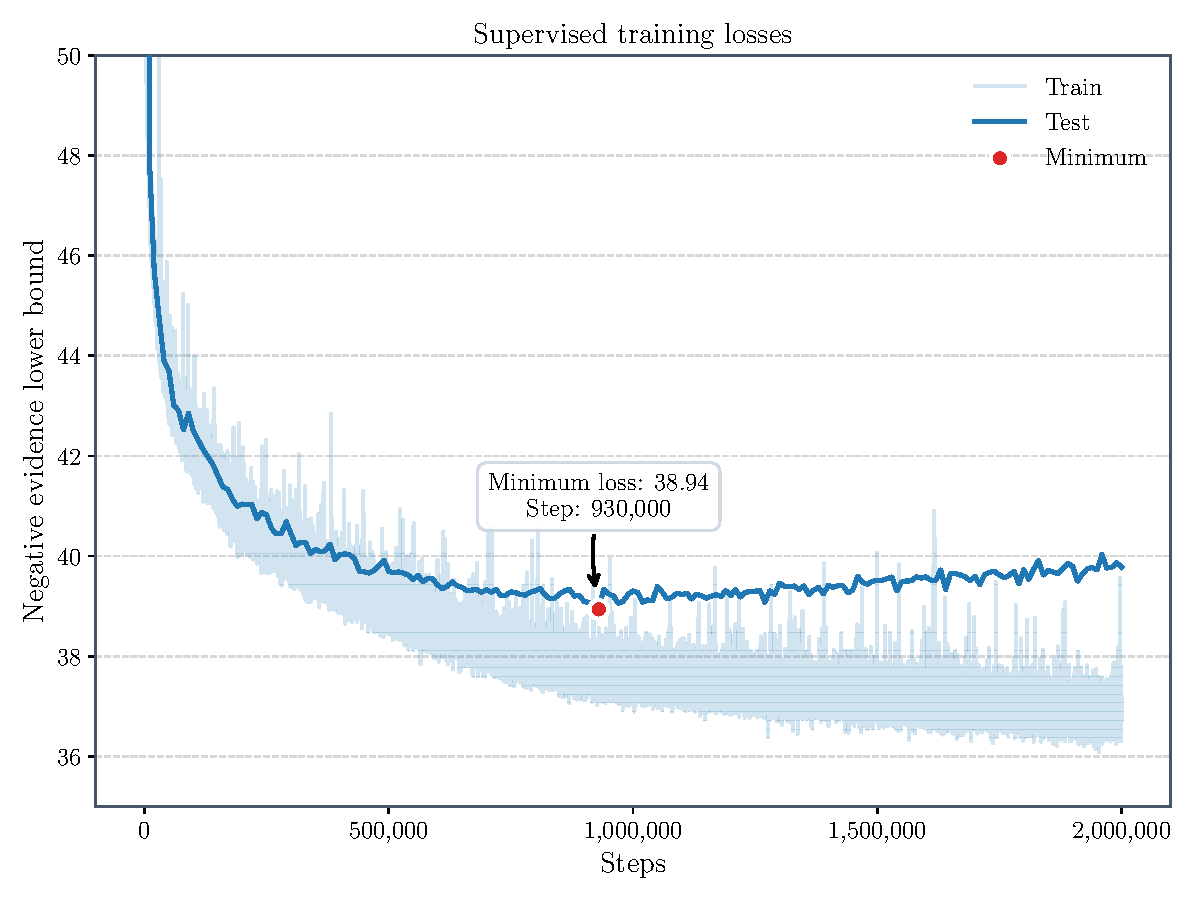
\includegraphics[width=\textwidth]{./sections/figures/supervised_training_progress/Training_loss.pdf}
    \caption{The negative evidence lower bound as a function of the training steps. After around 1,000,000, we observe clear overfitting.}
    \label{fig:training_loss}
\end{figure}

As described in section \ref{sec:evaluation criteria}, our main evaluation metric is the proportion of positions that pass both the uniqueness and the counter-intuitiveness criteria, i.e. the puzzle rate. Additionally, we monitor the legal rate, the uniqueness rate and the counter intuitiveness rate individually, as well as some diversity filtering metrics. In figure \ref{fig:supervised_training_metrics}, we see the evolution of these metrics over the supervised training run. Each data point is collected by sampling 10,000 positions from the model for each checkpoint, which are stored on 100,000-step intervals. We notice that the legal rate quickly improves to the final value, whereas the other metrics, which are more nuanced, take longer to improve. We see that the uniqueness rate steadily improves, however, the counter intuitiveness values and consequently the puzzle rate are quite noisy. This is due to the high variance of the counter-intuitiveness metric, which stems from Stockfish being great at finding the correct solutions very quickly.

In figure \ref{fig:supervised_training_metrics}, we see that the values of the different metrics increase over the training steps. \textcolor{red}{Talk about overfitting (context from test probably decreases somewhere)}

% \ref{sec:supervised training}


\begin{figure}[htbp]
    \centering
    
\includegraphics[width=0.49\linewidth]{sections/figures/supervised_training_progress/Legal_rate.pdf}
    \hfill
    
\includegraphics[width=0.49\linewidth]{sections/figures/supervised_training_progress/Uniqueness_rate.pdf}
    
    \vspace{0.5cm}
    
    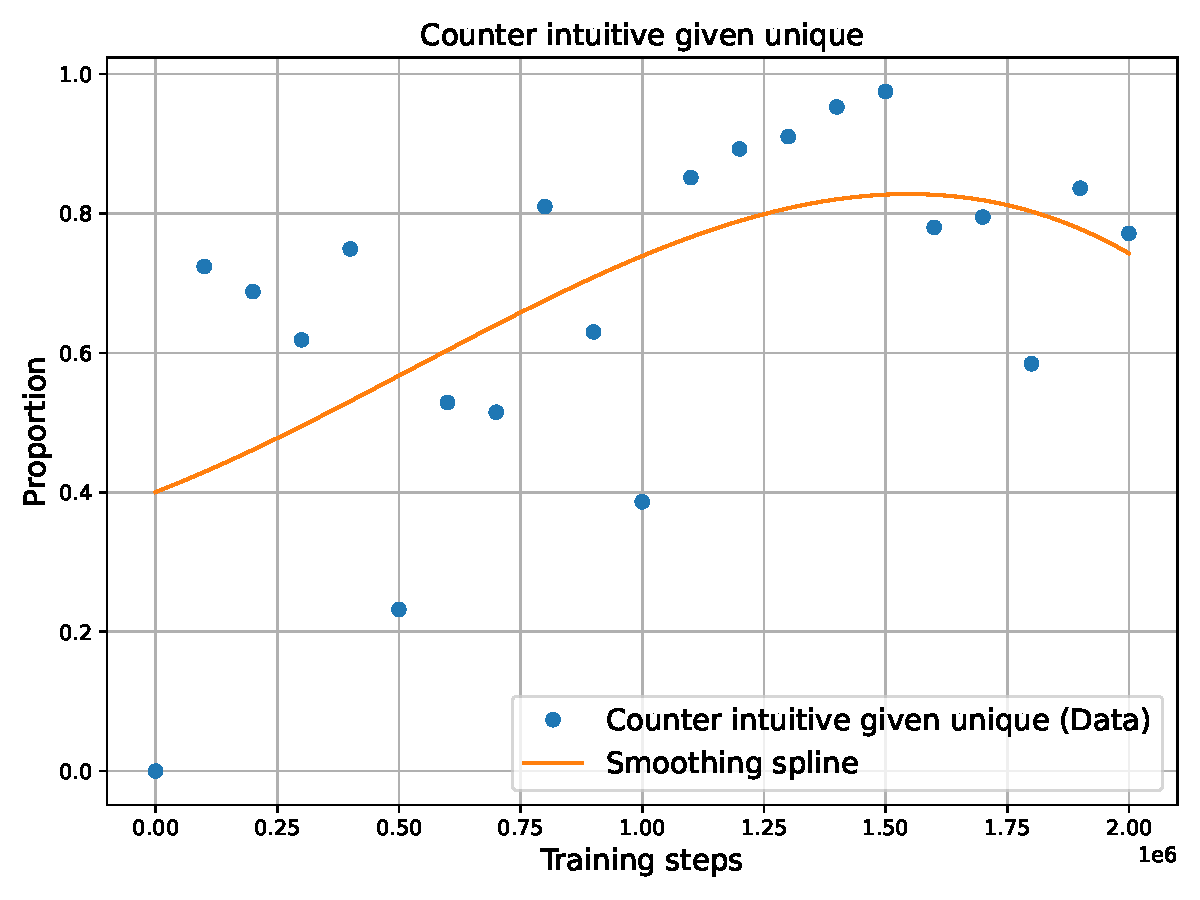
\includegraphics[width=0.49\linewidth]{sections/figures/supervised_training_progress/Counter_intuitive_given_unique.pdf}
    \hfill
    
\includegraphics[width=0.49\linewidth]{sections/figures/supervised_training_progress/Puzzle_rate.pdf}
    \caption{Evolution of the primary quality metrics with context from the training set during supervised pretraining.}
    \label{fig:supervised_training_metrics}
\end{figure}


\subsection{Reinforcement learning results}
\label{sec:rl results}





\subsection{Tests with the final model}
\label{sec:final tests}

\textcolor{red}{Example positions etc.}


\section{Conclusion}
\label{sec:conclusion}

% Discussion, limitations and future directions


% In this work, we explored using a masked diffusion model for the generation of chess puzzles. We followed the work of \citeauthor{feng2025generatingcreativechesspuzzles} and trained a masked diffusion model first with supervised training and later improved its performance by reinforcement learning. Additionally, we condition the generative process on the themes of a puzzle, for instance fork or mate-in-two, which steers the generation toward spesific puzzles. By supervised training we managed to train a model, which generates puzzles puzzles around $0.18\%$ of the time. We improve our model using reinforcement learning to generate puzzles around $0.37\%$ of the time. We also manage to improve the diversity of the generated positions.
%
% We had four main contributions from this research. Firstly, we demonstrated the effectiveness of masked diffusion models for generation of structured outputs. Secondly, we showed that the puzzle generation can be conditioned on specific themes. Thirdly, we demonstrated that the performance of masked diffusion models can be improved with reinforcement learning, although the task at hand is very difficult. Lastly, we demonstrated that the performance of the generation is improved by an auxiliary task of best move generation. Looking back at the contributions, although we have not demonstrated the generalization of these contributions to other tasks, in chess puzzle generation, the masked diffusion model works well and can be improved in many ways.
%
% For reinforcement learning, we employ an algorithm called DDPO. For this, we define a Markov decision process that works 
%
% For DDPO, we derive easy expressions for the step-wise KL divergence and the step-wise entropy.
%
% During this research, we have encountered many challenges. 
%
% This research has many limitations. (Generalizability, authors knowledge on chess etc.)
%
% In the future research, many questions remain. Firstly, we were unable to find a configuration, where the recently published ESPO algorithm would have worked. ESPO has offered benefits compared to DDPO in terms of efficiency and may improve the RL pipeline in this problem as well if a good configuration is found. Secondly, demonstrating similar setups in other NLP problems, and showcasing generalization, would push the research boundary further. Lastly, experimenting with different types of puzzle generation frameworks, such as combining iterative algorithms and generative models in one chain-of-thought \cite{wei2022chainofthought} system could improve puzzle generation and allow for easier generalization to other problems.
%
% \begin{itemize}
%     \item \textbf{Effectiveness of masked diffusion models:} Summarize how well the masked diffusion model performed at generating valid, structured chess puzzles compared to the baselines.
%     \item \textbf{Conditioning on themes:} Discuss the success rate of guiding the puzzle generation using specific tactical themes and any trade-offs observed (e.g., lower theme adherence after RL).
%     \item \textbf{Reinforcement learning improvements and challenges:} Highlight the increase in puzzle rate and counter-intuitiveness achieved through RL, but also mention the limitations encountered, such as mode collapse during extended training.
%     \item \textbf{Impact of auxiliary tasks:} Conclude on how predicting the best move simultaneously with the position improved the model's underlying chess knowledge and generative capabilities.
%     \item \textbf{Future directions:} Suggest applying this framework to other NLP tasks requiring strict structured outputs (like HTML rendering or code generation) and exploring better diversity filters or reward functions to prevent mode collapse in RL.
% \end{itemize}






% In this work, we explored using a masked diffusion model for the generation of chess puzzles, building upon the framework proposed by \citeauthor{feng2025generatingcreativechesspuzzles}. We initially trained a masked diffusion model using supervised training and subsequently enhanced its performance through reinforcement learning. A key aspect of our approach was conditioning the generative process on specific puzzle themes, effectively steering the generation toward desired puzzle types. After supervised training, our model successfully generated valid puzzles approximately $0.18\%$ of the time, although the puzzle rate changed a lot for each theme. By applying reinforcement learning, we more than doubled this success rate to around $0.37\%$, while simultaneously improving the diversity of the generated positions.

% We presented four main contributions in this research. First, we demonstrated the effectiveness of masked diffusion models for generating strict, structured outputs. Second, we showed that chess puzzle generation can be accurately conditioned on specific tactical themes. Third, we established that the performance of masked diffusion models can be meaningfully improved through reinforcement learning, despite the inherent difficulty of the task. Finally, we demonstrated that integrating the auxiliary task of predicting the best move alongside the position enhances the generative capabilities of the model. While we focused specifically on chess puzzle generation and did not demonstrate generalization to other tasks in this study, our results indicate that masked diffusion models can be very capable and offer various avenues for improvement in structured generation tasks.

% For the reinforcement learning phase, we employed the Denoising Diffusion Policy Optimization algorithm, which is extremely principled and theoretically grounded. To facilitate this, we formulated a Markov decision process following \citeauthor{black2024trainingdiffusionmodelsreinforcement}, which is suitable for the generation process. The MDP was formulated step-wise, which contrasts with the some of the latest dLLM research \cite{ou2025principledrldiffusionllms}. The states of the MDP were the partially unmasked token sequences and the actions were the generation of a new partially unmasked sequence. The transitions were deterministic and the rewards zero except for the last step where a nonzero reward was given to good puzzles and illegal positions. Additionally, we derived tractable expressions for the step-wise KL divergence and step-wise entropy, which are easy to compute and allow comparisons to traditional LLMs. With these expressions, we attempted to prevent model collapse and unrealistic positions.

% Despite the results, we encountered several challenges and limitations during this research. For instance, while we hope our findings are broadly applicable, we have not yet demonstrated the generalization of these contributions to other natural language processing tasks. Additionally, the manual evaluation and selection of the generated puzzles were inherently constrained by the author's level of chess knowledge. A stronger player or puzzle composer might offer a different perspective specifically to evaluation of our final model. Lastly, the stability and model collapse problems in reinforcement learning posed challenges to the algorithm we used. Connected to this, the decrease in theme match rate during RL may be caused by our theme match criterion, which is by no means the only way of defining a match. Perhaps, some combinations of themes allow the model to generate puzzles more often causing the model to converge to generating positions with the easy theme. These limitations leave room for further experimentation and studies.

% Looking ahead, numerous questions and directions for future research remain. During our experiments, we were unable to find a configuration where the recently published ESPO algorithm succeeded. Since algorithms that efficiently approximate the importance ratio have shown some benefits over DDPO \cite{ou2025principledrldiffusionllms, wang2026d2improvingresoning}, discovering a viable configuration could further optimize the RL pipeline for this problem. Furthermore, applying similar setups to other NLP domains to showcase generalizability would significantly advance the research boundary. Lastly, experimenting with alternative puzzle generation frameworks, such as combining iterative algorithms and generative models within a chain-of-thought system \cite{wei2022chainofthought}, could not only improve chess puzzle generation but also pave the way for easier adaptation to problems in other domains.

In this work, we explored using a masked diffusion model for the generation of chess puzzles, building upon the framework proposed by \citeauthor{feng2025generatingcreativechesspuzzles}. We initially trained a masked diffusion model using supervised training and subsequently enhanced its performance through reinforcement learning. A key aspect of our approach was conditioning the generative process on specific puzzle themes, effectively steering the generation toward desired puzzle types. After supervised training, our model successfully generated valid puzzles approximately $0.18\%$ of the time, although the puzzle rate varied considerably across different themes. By applying reinforcement learning, we more than doubled this success rate to around $0.37\%$, while simultaneously improving the diversity of the generated positions.

We presented four main contributions in this research. First, we demonstrated the effectiveness of masked diffusion models for generating strict, structured outputs. Second, we showed that chess puzzle generation can be accurately conditioned on specific tactical themes. Third, we established that the performance of masked diffusion models can be meaningfully improved through reinforcement learning, despite the inherent difficulty of the task. Finally, we demonstrated that integrating the auxiliary task of predicting the best move alongside the position enhances the generative capabilities of the model. While we focused specifically on chess puzzle generation and did not demonstrate generalization to other tasks in this study, our results indicate that masked diffusion models are highly capable and offer various avenues for improvement in structured generation tasks.

For the reinforcement learning phase, we employed the Denoising Diffusion Policy Optimization algorithm, an approach that is highly principled and theoretically grounded. To adapt this algorithm for our task, we formulated a Markov decision process following the methodology of \citeauthor{black2024trainingdiffusionmodelsreinforcement}. Crucially, our MDP was formulated step-wise, which contrasts with some of the latest research in discrete large language models \cite{ou2025principledrldiffusionllms, rojas2025improvingreasoningdiffusionlanguage}. In this setup, the states correspond to the partially unmasked token sequences, while the actions define the generation of the subsequent partially unmasked sequence. The transitions between states are deterministic, and the rewards remain zero until the final step, at which point a non-zero reward is assigned based on the quality of the puzzle. To further stabilize the training process, we derived tractable expressions for the step-wise KL divergence and step-wise entropy. These expressions allowed a direct comparison to traditional autoregressive LLMs, and served as vital regularization tools to prevent model collapse and the generation of unrealistic positions.

Despite our results, we encountered several challenges and limitations during this research. For instance, while we hope our findings are broadly applicable, we have not yet demonstrated the generalization of these contributions to other natural language processing tasks. Additionally, the manual evaluation and selection of the generated puzzles were inherently constrained by the author's level of chess knowledge. A stronger chess player or puzzle composer might offer a different perspective specifically regarding the evaluation of our final model. Furthermore, stability issues and model collapse during reinforcement learning posed significant challenges to our chosen algorithm. Relatedly, the observed decrease in the theme match rate during RL may stem from our specific theme match criterion, which is by no means the only way to define a successful match. It is possible that certain theme combinations inherently allow the model to generate puzzles more easily, causing it to converge toward generating positions that favor these "easier" themes. These limitations highlight clear avenues for further experimentation and study.

Looking ahead, numerous questions and directions for future research remain. During our experiments, we were unable to find a configuration where the recently published ESPO algorithm succeeded. Since algorithms that efficiently approximate the importance ratio have shown benefits over DDPO \cite{ou2025principledrldiffusionllms, wang2026d2improvingresoning}, discovering a viable ESPO configuration could further optimize the RL pipeline for this problem. Furthermore, applying similar setups to other NLP domains to showcase generalizability would significantly advance the research boundary. Lastly, experimenting with alternative puzzle generation frameworks, such as combining iterative algorithms and generative models within a chain-of-thought system \cite{wei2022chainofthought}, could not only improve chess puzzle generation but also pave the way for easier adaptation to complex problems in other domains.

\section*{AI disclosure}

During this work, large language models (primarily Gemini 3.1 Pro and Gemini 3.5 Flash with both the web interface and Google Antigravity) were utilized to assist with programming tasks and text refinement. The author takes full responsibility for the entirety of this work, encompassing all experiments, software implementations, figures, tables, and written content. All output generated with AI assistance was manually reviewed and explicitly approved by the author. Furthermore, all architectural decisions in the software, as well as the choices regarding the thesis content, were made by the author, supported by the guidance of advisor Eric Malmi, supervisor Nuutti Hyvönen, and others.




\bibliography{references.bib}



\clearpage
\thesisappendix

\section{Theme computation}
\label{sec:theme computation}

To identify the tactical themes present in a generated position, we employ the Lichess puzzler pipeline \cite{lichesspuzzler}, which iterates over the principal variation to detect specific themes. We group these themes into several distinct categories, which include the following: state of game, type of endgame, type of checkmate, length of checkmate, length of puzzle, winning states, and other tactics. Table \ref{tab:themes} enumerates every specific theme we evaluate during the puzzle evaluation process. While the Lichess puzzles dataset \cite{lichesspuzzledatabase} contains additional metadata tags, we exclusively focus on objective, position-based themes. We intentionally discard the other tags, such as ``master vs. master'', as they cannot be verified from the board state alone.

During reinforcement learning and evaluation, we determine whether a generated puzzle successfully matches the requested conditions by comparing the generated theme set $\mathcal{T}_{\text{gen}}$ against the requested theme set $\mathcal{T}_{\text{req}}$. Rather than requiring a strict superset match $\mathcal{T}_{\text{req}} \subseteq \mathcal{T}_{\text{gen}}$, we use the specific groups for the check. The complete theme matching logic is detailed in Algorithm \ref{alg:theme match}.

\begin{table}[h]
    \centering
    \renewcommand{\arraystretch}{1.3}
    \begin{tabular}{l p{10cm}}
        \hline
        \textbf{Category} & \textbf{Themes} \\
        \hline
        State-of-game & Opening, Middlegame, Endgame \\
        Type-of-endgame & Pawn endgame, Bishop endgame, Knight endgame, Rook endgame, Queen endgame, Queen rook endgame \\
        Type-of-checkmate & Mate, Back rank mate, Boden mate, Smothered mate, Hook mate, Double bishop mate, Arabian mate, Dovetail mate, Anastasia mate \\
        Length-of-checkmate & Mate in 1, Mate in 2, Mate in 3, Mate in 4, Mate in 5 \\
        Length-of-puzzle & One move, Short, Long, Very long \\
        Winning & Crushing, Advantage \\
        Other & Hanging piece, Fork, Interference, Kingside attack, Zugzwang, Exposed king, Skewer, Pin, Quiet move, Discovered attack, Sacrifice, Deflection, Advanced pawn, Attraction, Promotion, Queenside attack, Defensive move, Attacking f2/f7, Clearance, Intermezzo, Equality, Trapped piece, X-ray attack, Capturing defender, Double check, En passant, Castling, Underpromotion \\
        \hline
    \end{tabular}
    \caption{The complete list of themes supported by the Lichess puzzler pipeline, grouped by their respective categories.}
    \label{tab:themes}
\end{table}

\begin{algorithm}[H]
    \caption{Themes match}
    \label{alg:theme match}
    \begin{algorithmic}
        \Require Requested themes $\mathcal{T}_{\text{req}}$, Generated puzzle themes $\mathcal{T}_{\text{gen}}$
        \Require Category sets $\mathcal{S}_{\text{state}}$, $\mathcal{S}_{\text{endgame}}$, $\mathcal{S}_{\text{mate\_len}}$, $\mathcal{S}_{\text{mate\_type}}$, $\mathcal{S}_{\text{other}}$
        
        \If{$(\mathcal{T}_{\text{req}} \cap \mathcal{S}_{\text{state}}) \not\subseteq \mathcal{T}_{\text{gen}}$}
            \State \textbf{return} False
        \EndIf
        
        \If{\text{``endgame''} $\in \mathcal{T}_{\text{req}}$}
            \If{$(\mathcal{T}_{\text{req}} \cap \mathcal{S}_{\text{endgame}}) \not\subseteq \mathcal{T}_{\text{gen}}$}
                \State \textbf{return} False
            \EndIf
        \EndIf
        
        \If{\text{``mate''} $\in \mathcal{T}_{\text{req}}$}
            \If{\text{``mate''} $\notin \mathcal{T}_{\text{gen}}$}
                \State \textbf{return} False
            \EndIf
            \If{$(\mathcal{T}_{\text{req}} \cap \mathcal{S}_{\text{mate\_len}}) \not\subseteq \mathcal{T}_{\text{gen}}$}
                \State \textbf{return} False
            \EndIf
            \If{$(\mathcal{T}_{\text{req}} \cap \mathcal{S}_{\text{mate\_type}}) \not\subseteq \mathcal{T}_{\text{gen}}$}
                \State \textbf{return} False
            \EndIf
        \Else
            \If{$(\mathcal{T}_{\text{req}} \cap \mathcal{S}_{\text{other}}) \not\subseteq \mathcal{T}_{\text{gen}}$}
                \State \textbf{return} False
            \EndIf
        \EndIf
        
        \State \textbf{return} True
    \end{algorithmic}
\end{algorithm}




\section{Supervised training}


In addition to the training metrics presented in Figure \ref{fig:supervised_training_metrics}, we also monitor the model's performance during supervised training by evaluating generated samples conditioned on themes drawn from the held-out test set. These test-set evaluation metrics are illustrated in Figure \ref{fig:supervised_training_test_metrics}. We observe that while the legal rate and uniqueness rate saturate after approximately 1,000,000 training steps, the counter-intuitiveness and overall puzzle rates converge significantly faster. However, the inherent variance in the counter-intuitiveness metric makes identifying the precise convergence point of the puzzle rate challenging. We observe that the performance of these metrics do not decrease similarly to the test loss in Figure \ref{fig:training_loss}. We still select the checkpoint at 1,000,000 training steps, as the metrics do not improve with more training.

\begin{figure}[h]
    \centering
    
\includegraphics[width=0.49\linewidth]{sections/figures/supervised_training_progress/test/Legal_rate.pdf}
    \hfill
    
\includegraphics[width=0.49\linewidth]{sections/figures/supervised_training_progress/test/Uniqueness_rate.pdf}
    
    \vspace{0.5cm}
    
    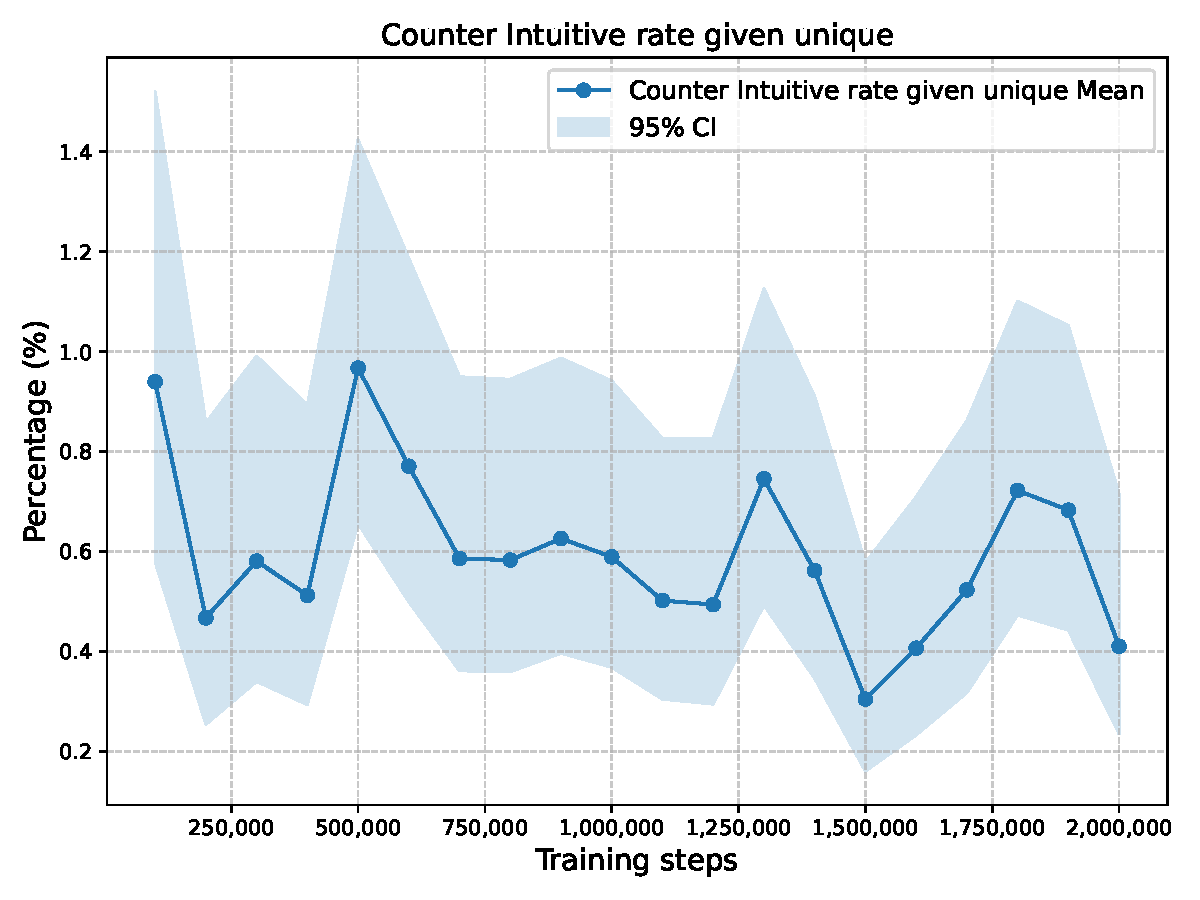
\includegraphics[width=0.49\linewidth]{sections/figures/supervised_training_progress/test/Counter_intuitive_rate_given_unique.pdf}
    \hfill
    
\includegraphics[width=0.49\linewidth]{sections/figures/supervised_training_progress/test/Puzzle_rate.pdf}
    \caption{Evolution of the primary quality metrics with context from the testing set during supervised pretraining.}
    \label{fig:supervised_training_test_metrics}
\end{figure}


To further benchmark our the performance of our model, we additionally sample from the model with a lower temperature of 0.1 \ref{tab:supervised metrics low temperature}. We notice that with the almost greedy sampling, the uniqueness is considerably improved, whereas, the counter-intuitiveness is not. Furthermore, the difference between the move sampling is further amplified, as if we sample the move after sampling the position, the uniqueness is considerably lower than if the move was sampled simultaneously to the position. We conclude that the best move prediction improves the model performance meaningfully. This improvement comes at a cost to the distance metrics though, as the board distance to the Lichess dataset is around 6.91 and the PV distance is 0.80 when sampling with a low temperature.

\begin{table}[h]
    \centering
    \caption{The final metrics after supervised training with different context distributions. The sampling is performed with a temperature $0.1$ and $256$ denoising steps.}
    \resizebox{\textwidth}{!}{
    \begin{tabular}{|c|c|c|c|c|c|c|}
        \hline
        Context & Sampling & Legal & Unique & Counter-intuitive | unique & Puzzle & Theme\\
        \hline\hline
        Train & block & 98.04 $\pm$ 0.27 & 35.20 $\pm$ 0.93 & 0.50 $\pm$ 0.081 & 0.18 $\pm$ 0.081 & 90.18 $\pm$ 0.90 \\
        Train & normal & 99.44 $\pm$ 0.14 & 42.01 $\pm$ 0.96 & 0.63 $\pm$ 0.099 & 0.26 $\pm$ 0.099 & 92.75 $\pm$ 0.94 \\
        Test & block & 98.33 $\pm$ 0.25 & 34.89 $\pm$ 0.92 & 0.50 $\pm$ 0.081 & 0.18 $\pm$ 0.081 & 89.98 $\pm$ 0.90 \\
        Test & normal & 99.45 $\pm$ 0.14 & 42.37 $\pm$ 0.96 & 0.48 $\pm$ 0.088 & 0.21 $\pm$ 0.088 & 92.90 $\pm$ 0.95 \\
        \hline\hline
        \multicolumn{2}{|c|}{Lichess puzzles} & \textbf{100.0} $\pm$ 0.0 & \textbf{83.58} $\pm$ 0.23 & \textbf{1.55} $\pm$ 0.070 & \textbf{1.29} $\pm$ 0.070 & \textbf{100.0} $\pm$ 0.0\\
        \hline
    \end{tabular}
    }
    \label{tab:supervised metrics low temperature}
\end{table}


\section{Reinforcement learning}
\label{sec:RL appendix}

\subsection{Additional results}

In this section, we present a few additional results on the reinforcement learning. We begin our experiments by training a model with using only the legality, uniqueness and counter-intuitiveness as the components of the reward. In Figure \ref{fig:rl_overfit_metrics}, we observe the results of such a training run. We observe that the model collapses after around 1700 training steps. For this run, we use a learning rate of $3\cdot10^{-5}$ with $\mu=2$ gradient updates per batch and 32 groups of 6 generations with the same themes. Compared to the results of \citeauthor{feng2025generatingcreativechesspuzzles}, we see that the masked diffusion model is more resistant to overfitting compared to an LLM and takes a lot longer to collapse. This is supported by the findings of \citeauthor{nie2025scalingmaskeddiffusionmodels}, although our results are for reinforcement learning, whereas their results concern pretraining.

\begin{figure}[h]  % ddpo/Ablations/no_diversity_filtering
    \centering
    \begin{subfigure}[t]{0.48\textwidth}
        \centering
        
\includegraphics[width=\textwidth]{sections/figures/rl_training_progress/overfit/reward.pdf}
        \caption{Reward over training steps.}
        \label{fig:overfit_reward}
    \end{subfigure}
    \hfill
    \begin{subfigure}[t]{0.48\textwidth}
        \centering
        
\includegraphics[width=\textwidth]{sections/figures/rl_training_progress/overfit/unique_and_counter_intuitive.pdf}
        \caption{Puzzle rate over training steps.}
        \label{fig:overfit_unique}
    \end{subfigure}
    \vspace{0.5cm}
    \begin{subfigure}[t]{0.48\textwidth}
        \centering
        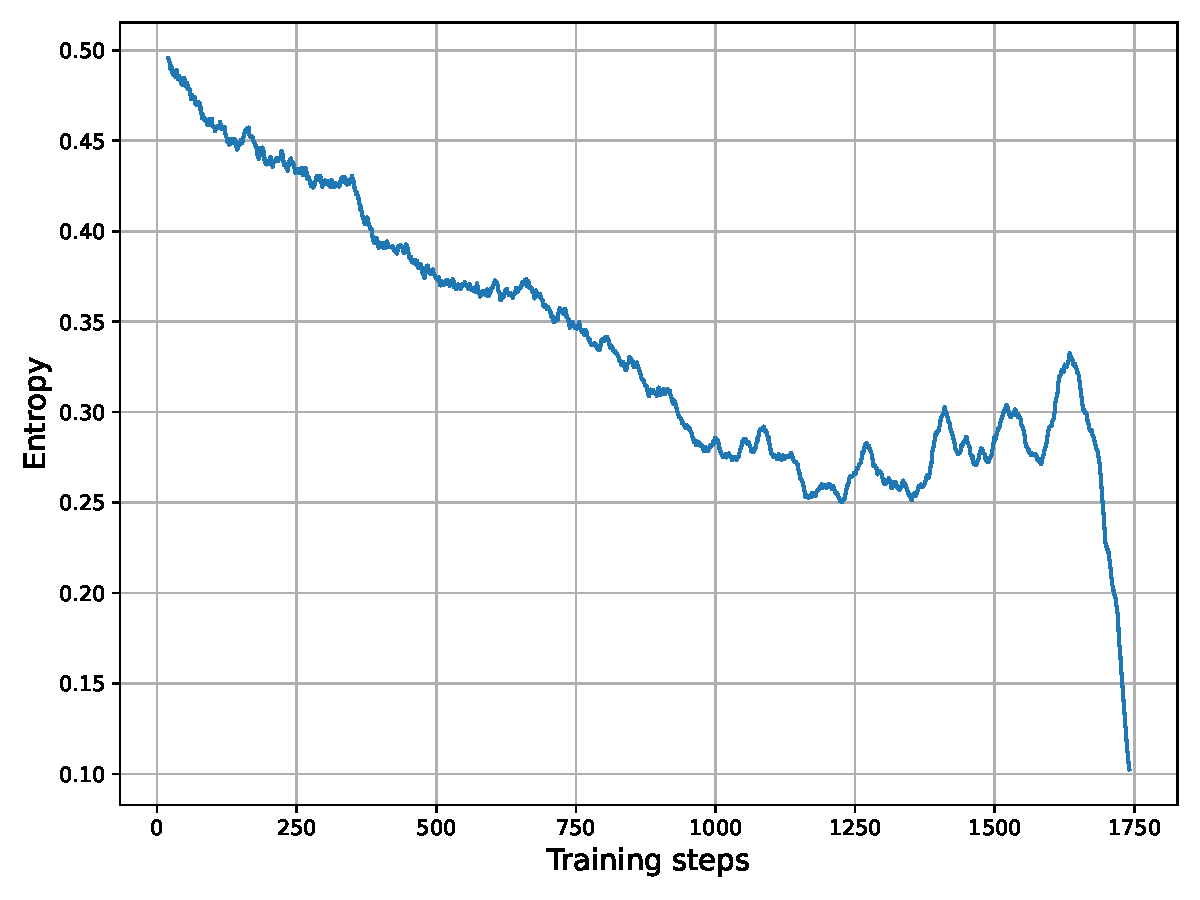
\includegraphics[width=\textwidth]{sections/figures/rl_training_progress/overfit/entropy.pdf}
        \caption{Entropy over training steps.}
        \label{fig:overfit_entropy}
    \end{subfigure}
    \hfill
    \begin{subfigure}[t]{0.48\textwidth}
        \centering
        
\includegraphics[width=\textwidth]{sections/figures/rl_training_progress/overfit/kl_divergence.pdf}
        \caption{KL divergence over training steps.}
        \label{fig:overfit_kl}
    \end{subfigure}
    \caption{An illustration of DDPO training with just legality, uniqueness and counter-intuitiveness based reward. We observe model collapse at around 1700 training steps.}
    \label{fig:rl_overfit_metrics}
\end{figure}

To combat model collapse, we introduce many diversity filtering mechanisms inspired by \cite{feng2025generatingcreativechesspuzzles}. We introduce the methods described in section \ref{sec:reward function} and perform manual hyperparameter search for a good value of the entropy coefficient $\gamma$. In Figure \ref{fig:entropy coef search} we observe that with a high entropy bonus coefficient $\gamma = 0.3$, the task is too difficult for our model to learn, but with a lower entropy bonus coefficient $\gamma = 0.03$ or $\gamma = 0.06$, the entropy slowly decreases.

\begin{figure}[h]  % ddpo/Ablations/all_diversity_filtering_kl_entropy_with_grad, ddpo/Ablations/all_diversity_filtering_kl_entropy_with_grad_large_entropy_coef, ddpo/Ablations/all_diversity_filtering_kl_entropy_with_grad_medium_entropy_coef
    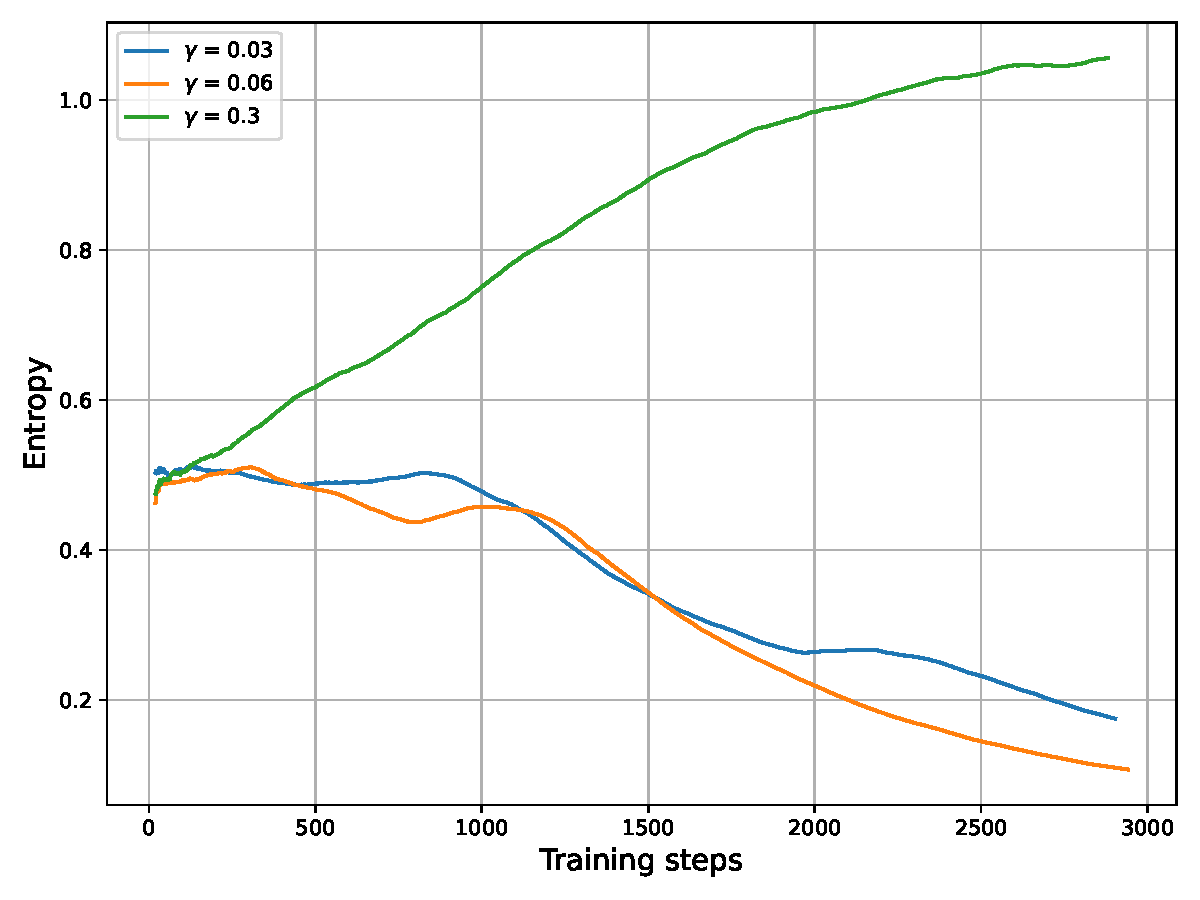
\includegraphics[width=0.49\textwidth]{sections/figures/rl_training_progress/overfit/DDPO/entropies.pdf}
    \hfill
    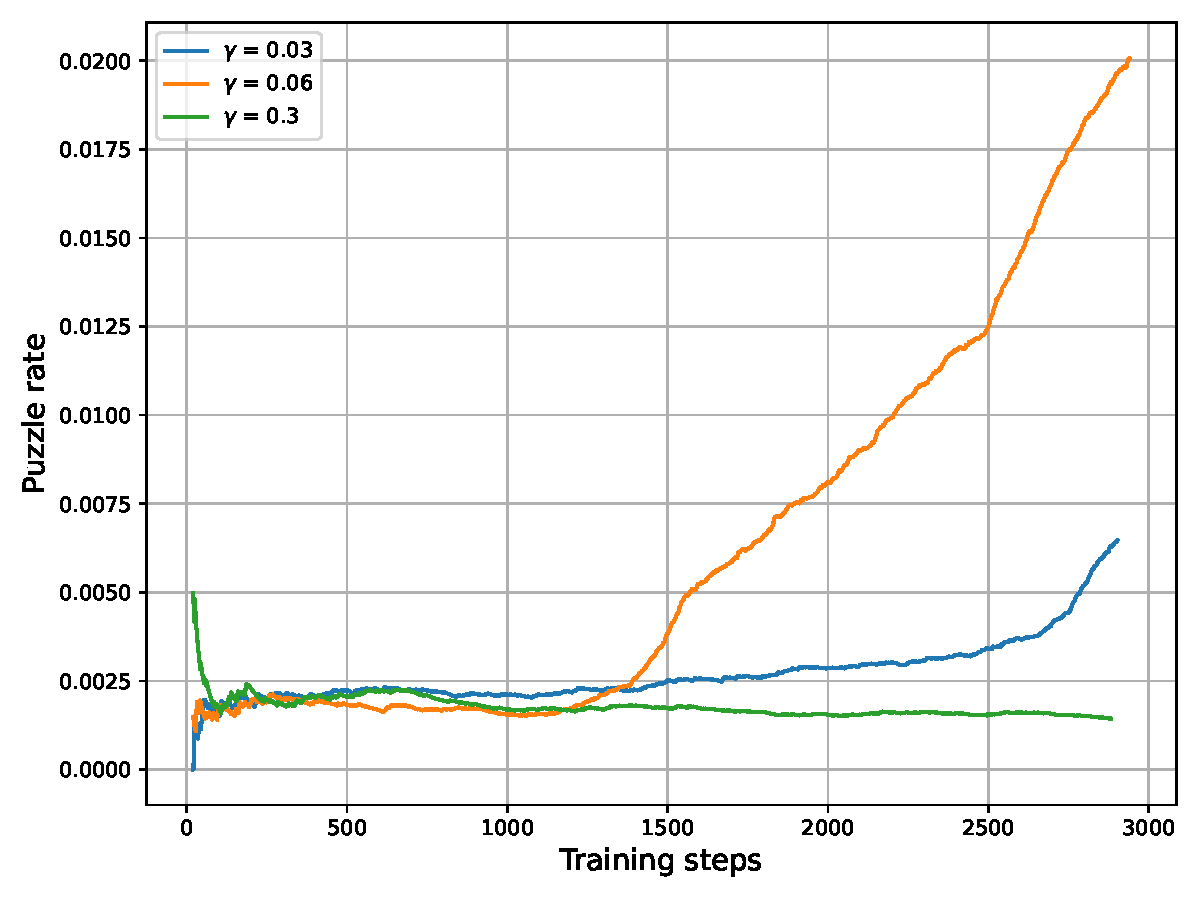
\includegraphics[width=0.49\textwidth]{sections/figures/rl_training_progress/overfit/DDPO/uniques_and_counter_intuitives.pdf}
    \caption{The training progress with different values of $\gamma$. We observe, that the two lower values overfit, whereas, the larger one does not learn.}
    \label{fig:entropy coef search}
\end{figure}


In Figures \ref{fig:theme_dist}, we present the distributions of themes in the lichess dataset as well as the generated positions. In Figure \ref{fig:ci_over_themes}, we present the counter-intuitive rates for each of these themes. We notice that it is considerably more difficult to generate counter-intuitive positions. For instance, although mate-in-one puzzles are quite common, no counter-intuitive mate-in-ones are present in the Lichess dataset or the generated positions.


\begin{figure}[h]
    \centering
    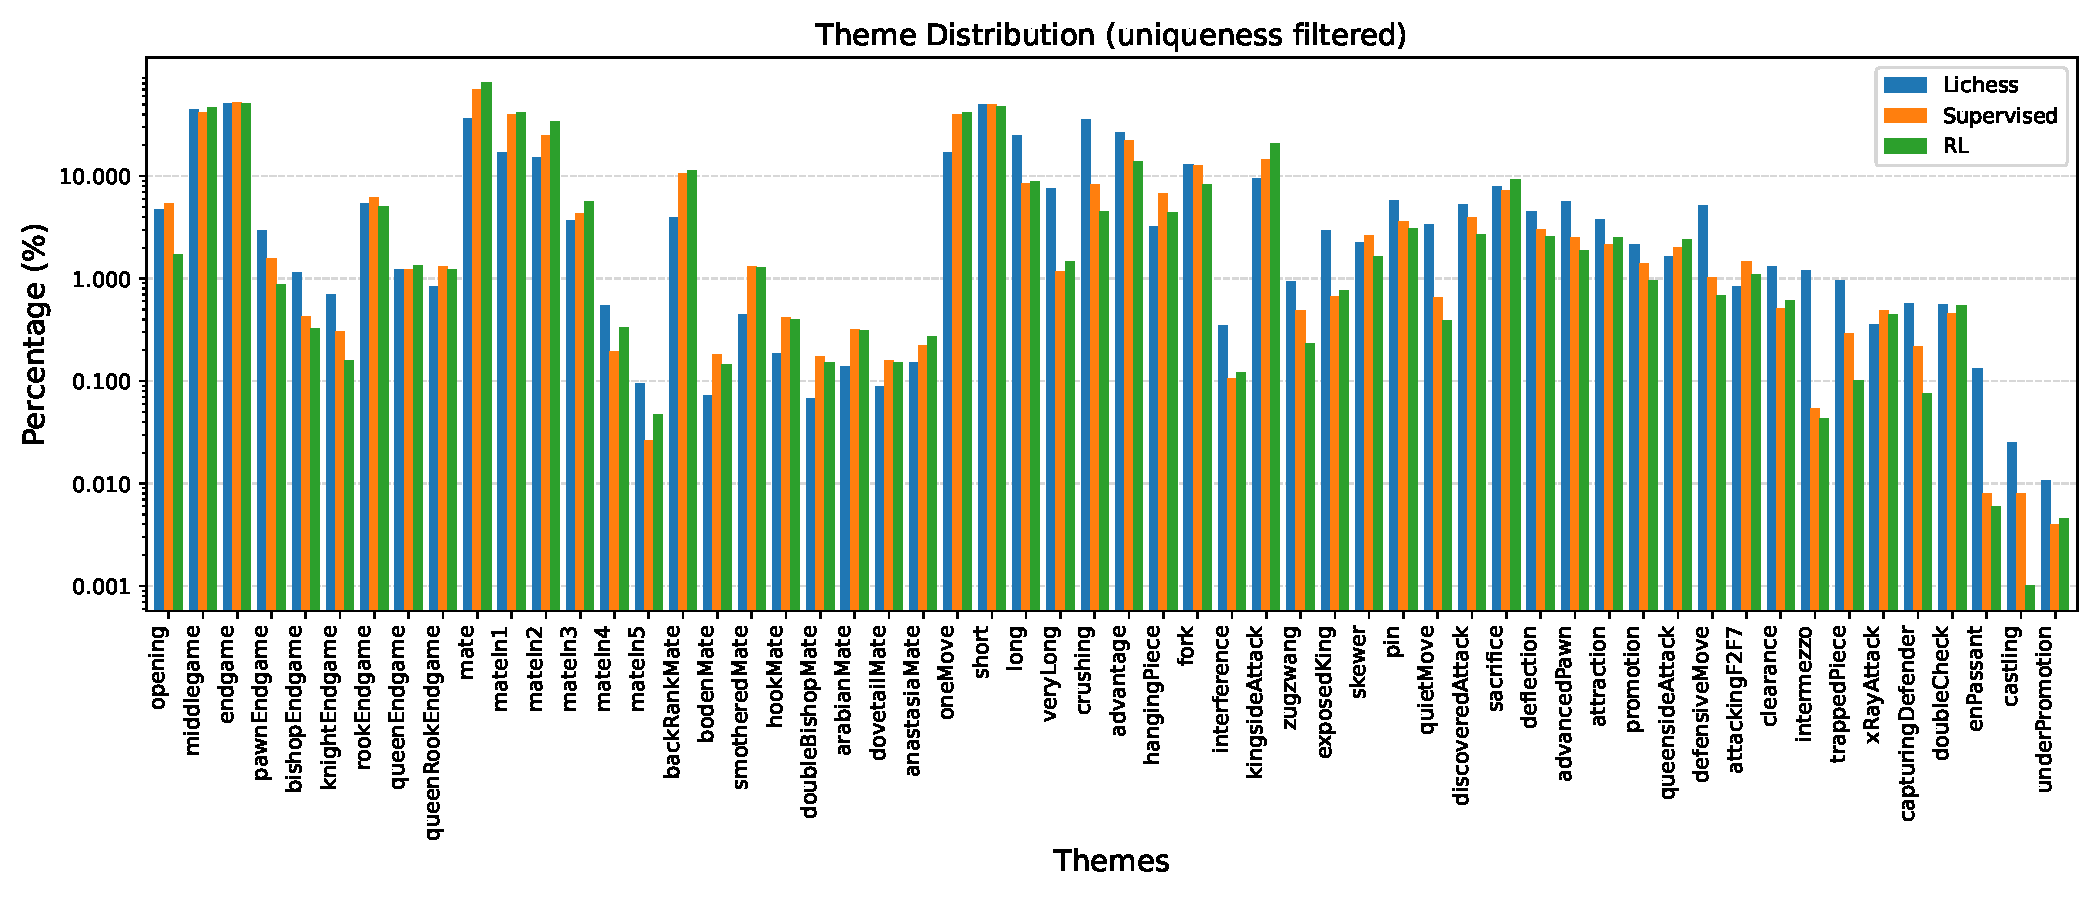
\includegraphics[width=\textwidth]{sections/figures/other/theme_distribution.pdf}
    \caption{The distribution of themes for the Lichess puzzles dataset, our supervised model and the final model. All positions are first filtered for positions with a unique solutions and the percentages are computed accross the filtered dataset.}
    \label{fig:theme_dist}
\end{figure}

\begin{figure}[h]
    \centering
    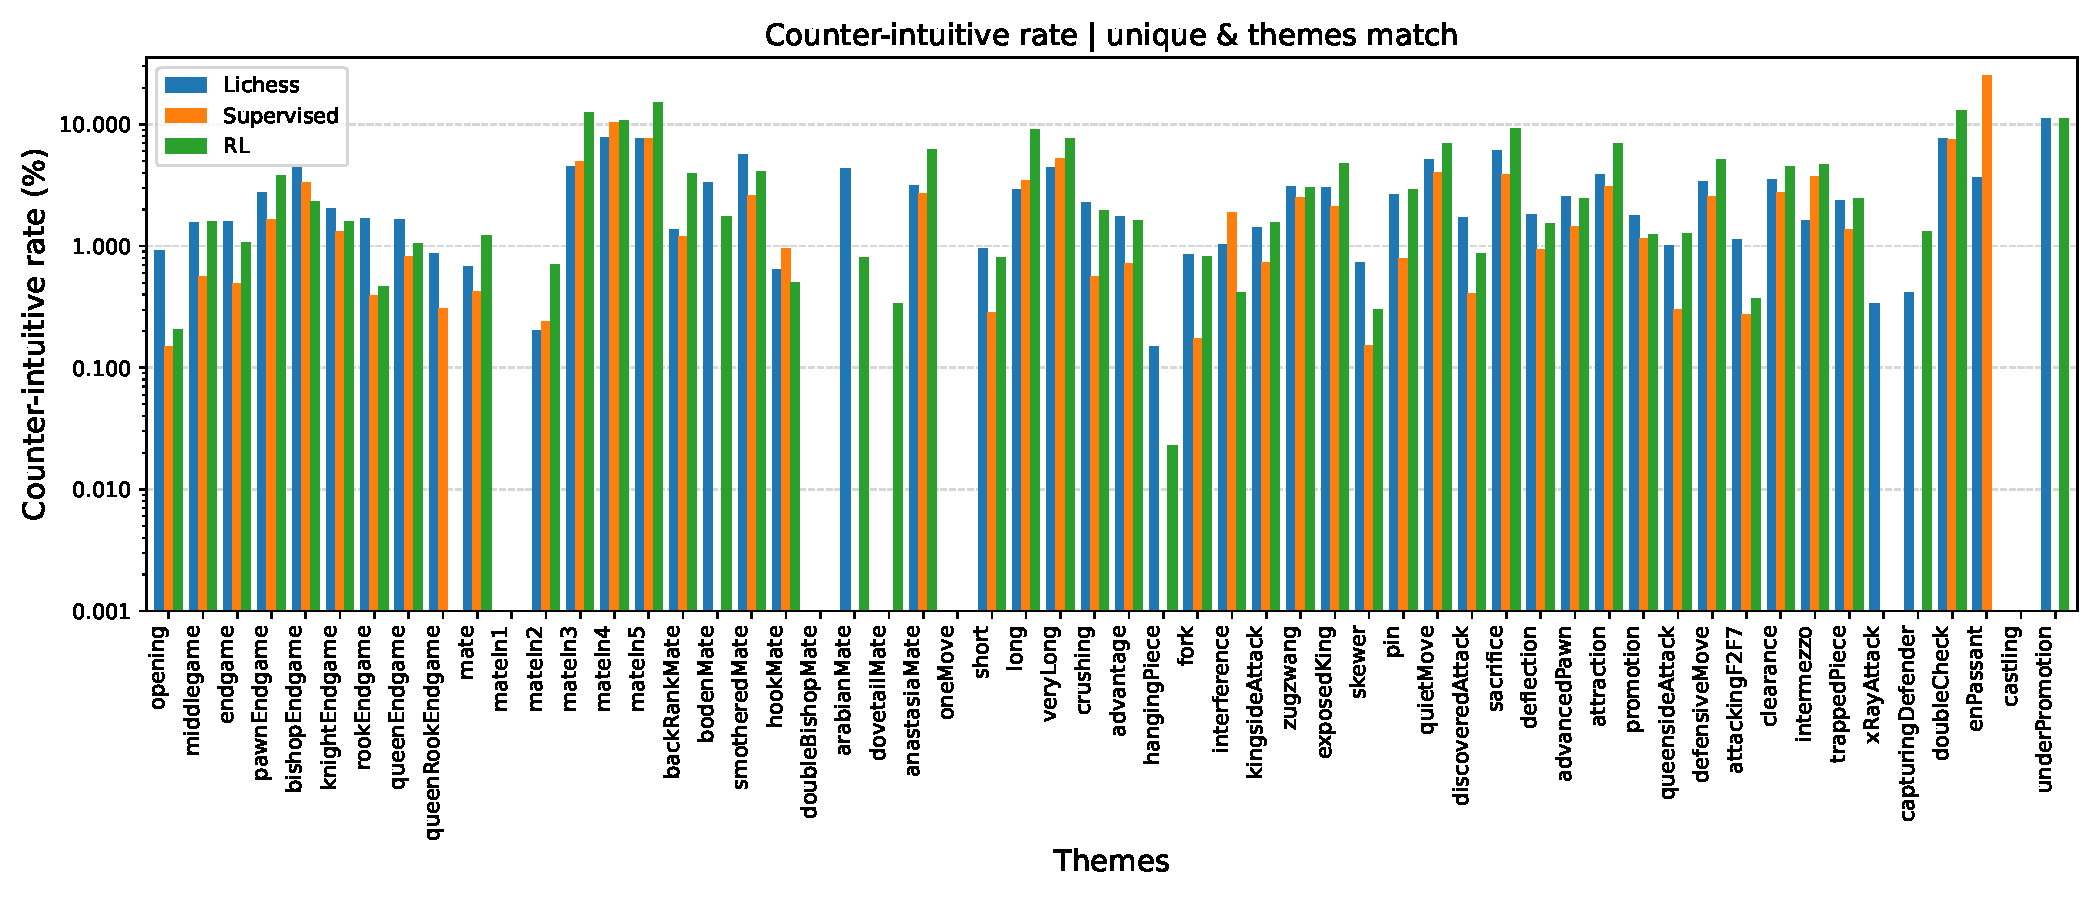
\includegraphics[width=\textwidth]{sections/figures/other/ci_distribution_over_themes.pdf}
    \caption{The counter-intuitive rate for the Lichess puzzles dataset, our supervised model and the final model accross all themes. All positions are first filtered for positions with a unique solutions and so that the themes match the ones the model was conditioned on and the percentages are computed accross the filtered dataset.}
    \label{fig:ci_over_themes}
\end{figure}



\subsection{ELBO-based Sequence-level Policy Optimization}

Before deciding to use DDPO, we attempt to use the ELBO-based sequence-level policy optimization (ESPO) algorithm \cite{ou2025principledrldiffusionllms}. ESPO is an algorithm specifically designed for masked diffusion language models, which led us to consider it first. Although we found some promising results, we were unable to get the model to learn effectively. In Figure \ref{fig:rl_overfit_metrics_ESPO}, we see that we are able to make the model find a puzzle, which produces high rewards, however, after introducing diversity filtering and other reward components, the model either marginally improved without meaningful progress or collapsed to illegal positions depending on the exact configuration. Interestingly, in Figure \ref{fig:rl_overfit_metrics_ESPO}, the model collapse happens quite a lot faster than for DDPO in Figure \ref{fig:rl_overfit_metrics} despite us using a lower learning rate $3\cdot10^{-6}$ with $\mu = 8$. We suspect the faster collapse could be related to ESPO making more efficient updates due to the sequence-level nature of the algorithm.

\begin{figure}[h]  % test/run6
    \begin{subfigure}[t]{0.48\textwidth}
        \centering
        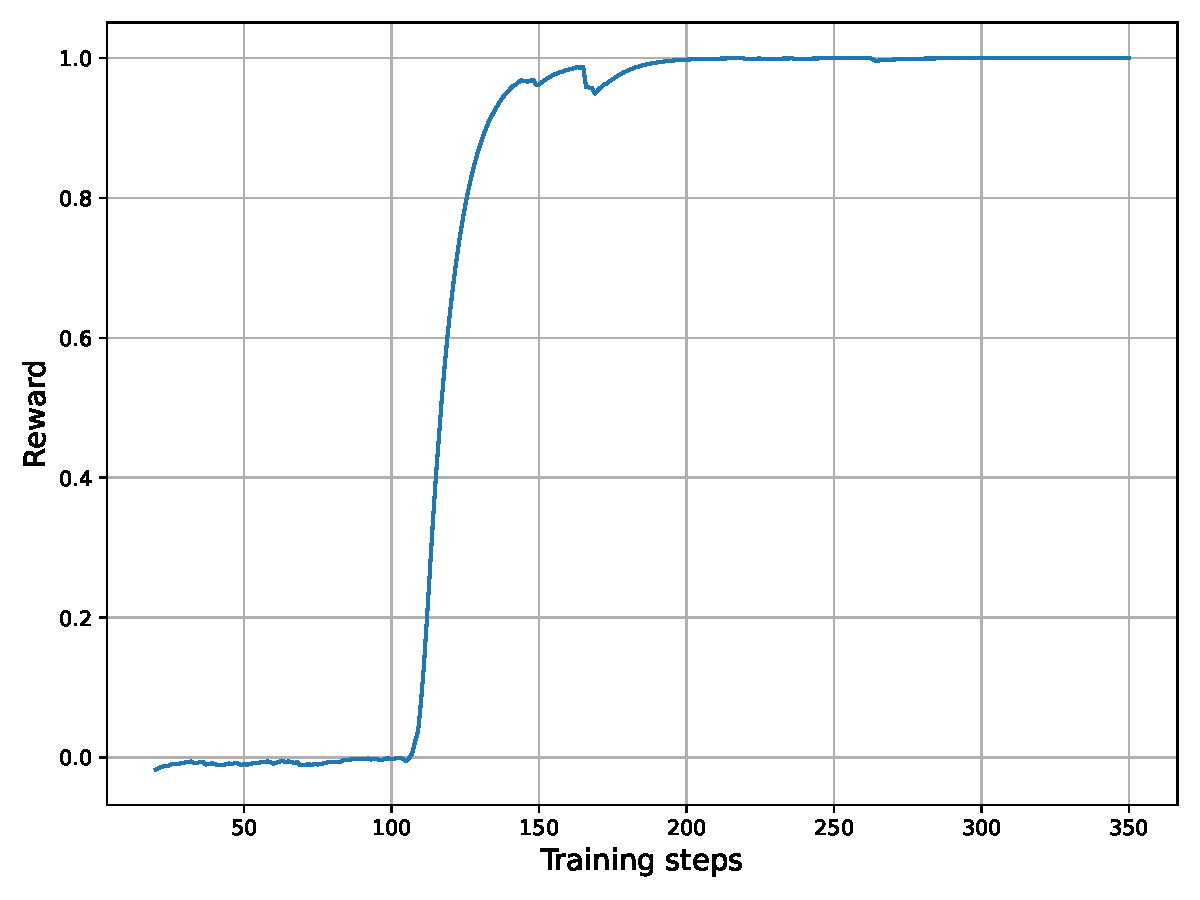
\includegraphics[width=\textwidth]{sections/figures/rl_training_progress/overfit/ESPO/reward.pdf}
        \caption{Reward over training steps.}
        \label{fig:overfit_entropy_ESPO}
    \end{subfigure}
    \hfill
    \begin{subfigure}[t]{0.48\textwidth}
        \centering
        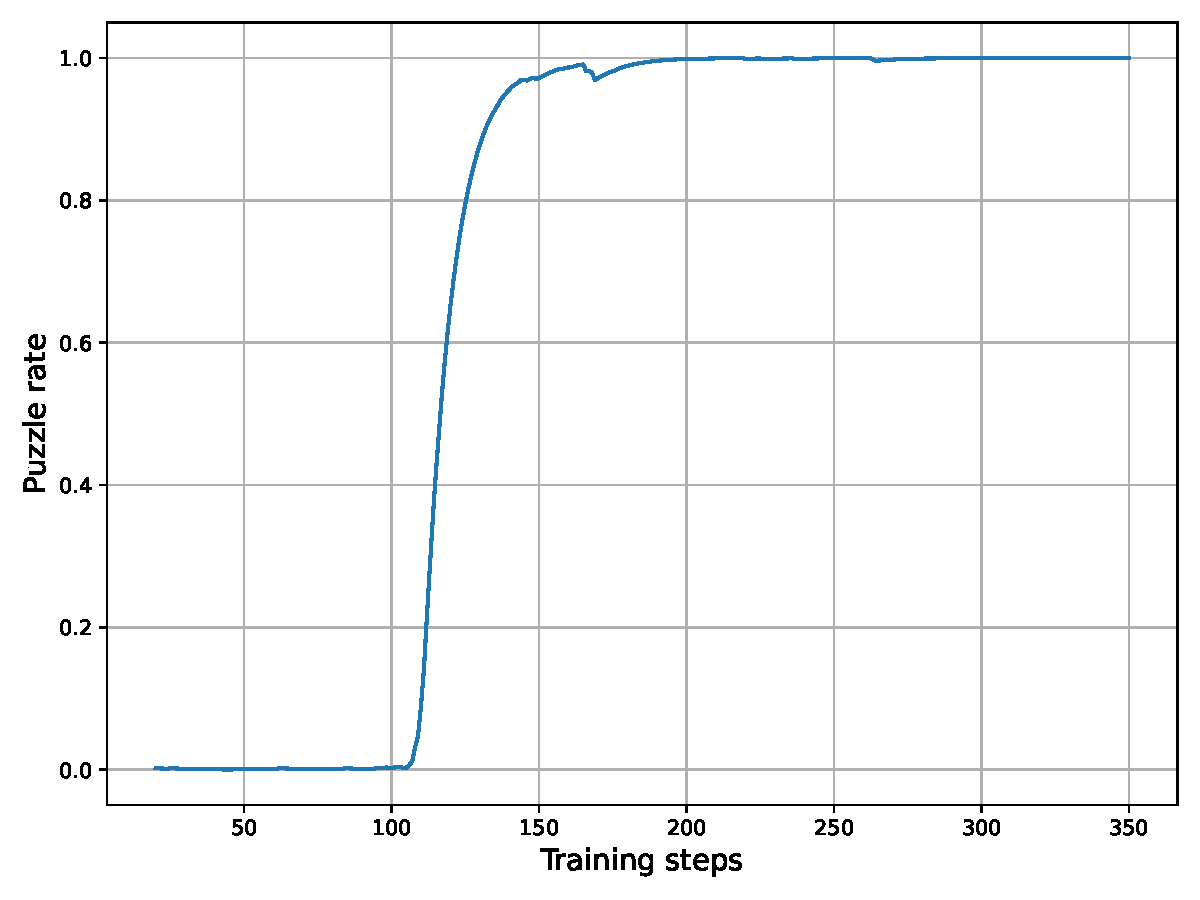
\includegraphics[width=\textwidth]{sections/figures/rl_training_progress/overfit/ESPO/unique_and_counter_intuitive.pdf}
        \caption{Puzzle rate over training steps.}
        \label{fig:overfit_kl_ESPO}
    \end{subfigure}
    \caption{An illustration of ESPO training with just legality, uniqueness and counter-intuitiveness based reward. We observe model collapse at around 110 training steps.}
    \label{fig:rl_overfit_metrics_ESPO}
\end{figure}

After observing model collapse, we enable all diversity filtering mechanisms described in section \ref{sec:reward function}. In figure \ref{fig:espo collapse}, we observe that the model collapses to generate illegal positions. Although, the model improved in figure \ref{fig:rl_overfit_metrics_ESPO}, we observe no meaningful improvement in figure \ref{fig:espo collapse} even in the beginning of the training despite using the same training algorithm. At around 400 training steps, we observe huge gradient spikes and despite using gradient norm clipping, the model collapses to generate completely empty boards with no pieces. In addition to this run, we experimented with ESPO a lot, but were unable to get meaningful improvement to the model without complete mode collapse.

\begin{figure}  % final_thesis_experiments/overfit3_espo and final_thesis_experiments/overfit4_espo
    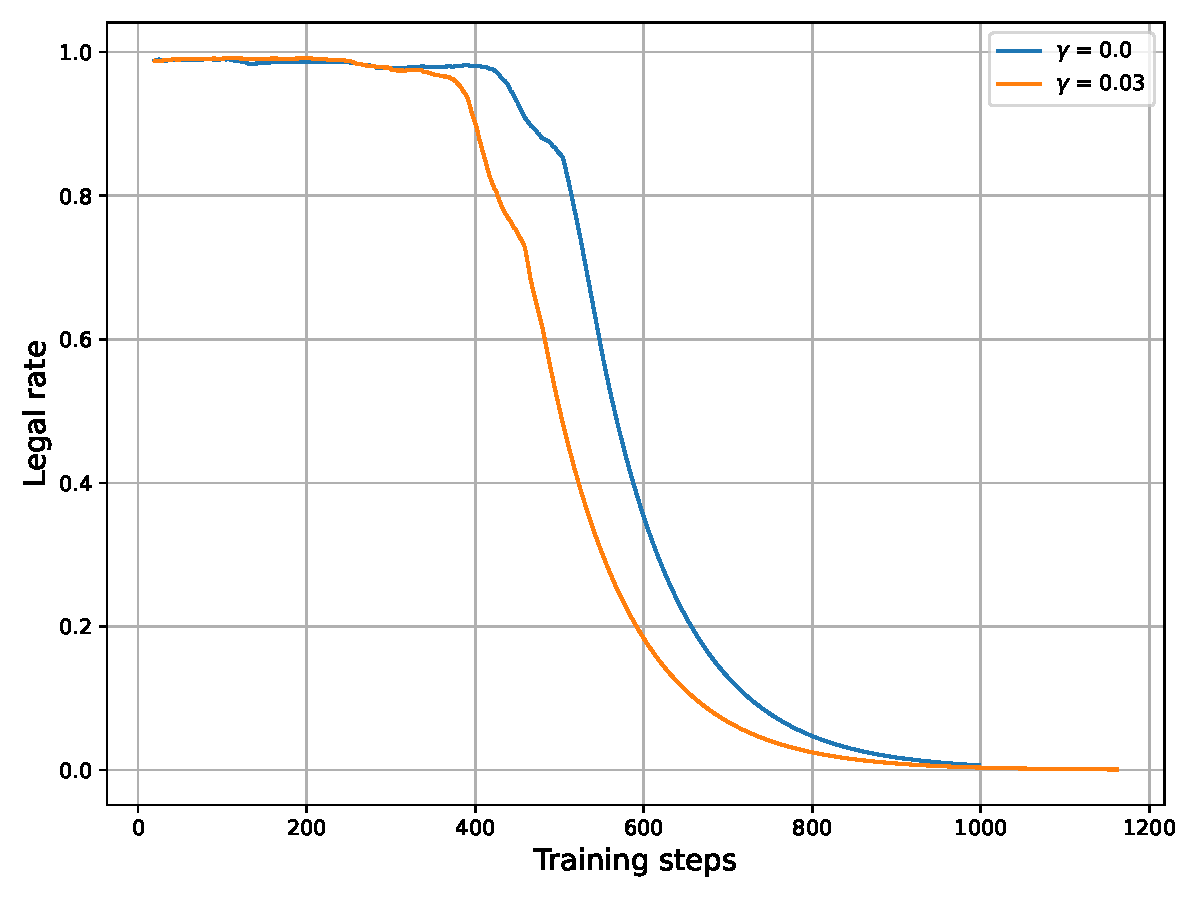
\includegraphics[width=0.49\textwidth]{sections/figures/rl_training_progress/overfit/ESPO/legal_rate.pdf}
    \hfill
    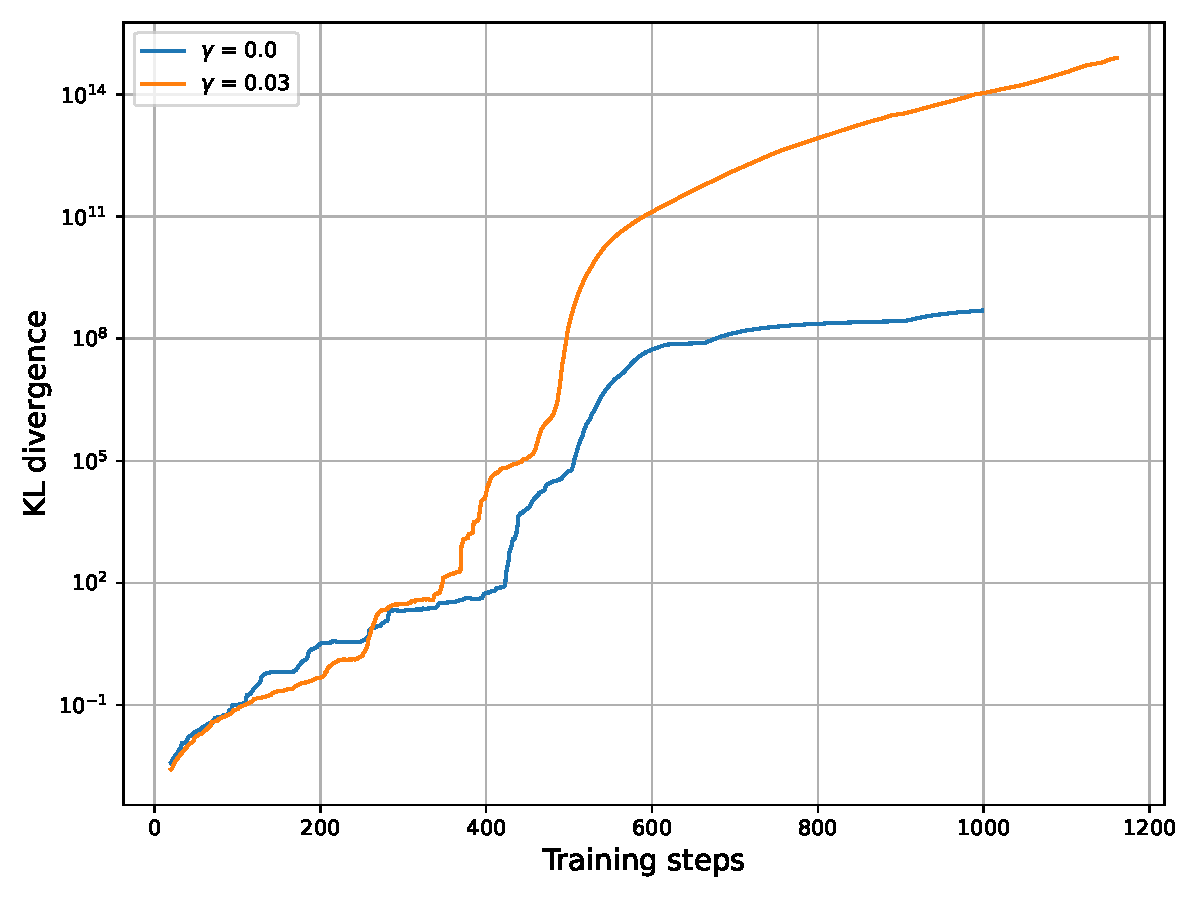
\includegraphics[width=0.49\textwidth]{sections/figures/rl_training_progress/overfit/ESPO/kl_divergence.pdf}
    \caption{The reinforcement learning training using ESPO with all diversity filtering mechanisms enabled. We observe that the model collapses and starts to generate illegal positions.}
    \label{fig:espo collapse}
\end{figure}





\section{Implementation details}
\label{sec:implementation details}

We provide an open-source implementation of the training algorithm we use at \url{https://github.com/naapeli/Generating-open-source-chess-puzzles}. All chess position evaluations were performed using the Stockfish engine \cite{stockfish}. To ensure reproducibility, we utilized a specific development build (dev-20260111-eb5a65ae), compiled on January 11, 2026, just before the release of Stockfish 18.


\end{document}
